\documentclass[a4paper,12pt]{article}

% Math
\usepackage{amsmath}
\usepackage{amsfonts}
\usepackage{amssymb}

% Graphics
\usepackage{booktabs}
\usepackage{graphicx}
\usepackage{caption}
\usepackage{subcaption}
\usepackage{float}
\usepackage{tikz}
\usetikzlibrary{arrows.meta, positioning}
\usepackage{pgfplots}
\pgfplotsset{compat=1.18}
\setlength{\marginparwidth}{1.7cm}
\setlength{\marginparsep}{0.3cm}
\usepackage[textsize=scriptsize]{todonotes}

% ==== Apa style ====
\usepackage[spanish,es-nodecimaldot]{babel}
\addto\captionsspanish{%
  \renewcommand{\tablename}{Tabla}%
  \renewcommand{\figurename}{Figura}%
}
%\usepackage{setspace}
\usepackage[utf8]{inputenc}

% Bibliography
\usepackage{csquotes}
\usepackage[style=apa, backend=biber]{biblatex}
\addbibresource{references.bib}

% Margins
\usepackage{geometry}
\geometry{left=2cm, right=2cm, top=2cm, bottom=2cm}

% comands
\newcommand{\bk}[1]{\left\langle #1 \right\rangle}
\newcommand{\set}[1]{\left\{#1\right\}}
\newcommand{\pti}[1]{\left.\frac{\partial #1}{\partial
x_i}\right|_{\vec x = \vec\mu}}
\newcommand{\ptj}[1]{\left.\frac{\partial #1}{\partial
x_j}\right|_{\vec x = \vec\mu}}
\newcommand{\ptij}[2]{\left.\frac{\partial #1}{\partial #2}\right|_{\vec\mu}}
% ======== hyperref ============
\usepackage{xcolor}
\usepackage[
  colorlinks=true,
  linkcolor=blue!60!black,
  citecolor=green!50!black,
  urlcolor=cyan!60!black,
  filecolor=magenta!60!black
]{hyperref}

\begin{document}
% ===== Portada institucional =====
\begin{titlepage}
\centering
{\Large UNIVERSIDAD NACIONAL DE PIURA}\\[4pt]
{\large FACULTAD DE CIENCIAS}\\[4pt]
{\large ESCUELA PROFESIONAL DE FÍSICA}\\[3cm]

{\Large\bfseries INFORME DE PRÁCTICAS PRE-PROFESIONALES}\\[6pt]
{\Large\bfseries METROLOGÍA Y ENSAYOS NO DESTRUCTIVOS}\\[3cm]

\begin{tabular}{ll}
ASESOR DE PRÁCTICAS & Dr. Francisco Arévalo Olivares\\[6pt]
ESTUDIANTE          & Rober Esbel Torres Tarrillo
\end{tabular}\\[3cm]

PIURA -- 2026
\end{titlepage}

% ===== Datos de la empresa =====
\newpage
{\centering
{\Large PHYSICS TECHNOLOGY INVESTIGATION (PHYTECHIN EIRL)}\\[1.5cm]

\begin{tabular}{ll}
RUC                       & 20525601952\\[6pt]
ACTIVIDADES DE LA EMPRESA & Metrología\\
                          & Ensayos no destructivos (END)\\
                          & Capacitaciones y asesorías\\[6pt]
GERENTE                   & Dr. Francisco Arévalo Olivares\\[6pt]
PERIODO DE PRÁCTICAS      & Por completar\\[6pt]
HORAS ACUMULADAS          & 300
\end{tabular}
\par}

\vspace{12pt}
\todo{Completar el periodo exacto de prácticas (el modelo de referencia indica
05 de agosto de 2025 -- 14 de mayo de 2026).}

\newpage
\tableofcontents
\newpage

\section{Introducción}

La metrología es la ciencia que establece las bases de la medición y garantiza que
los resultados obtenidos en el laboratorio o en la industria sean comparables,
confiables y trazables a patrones de referencia. En este contexto, la calibración
de instrumentos de medición constituye el procedimiento mediante el cual se
comprueba su comportamiento frente a un patrón de mayor exactitud, se cuantifican
sus errores de indicación y se estima la incertidumbre asociada conforme a la
guía GUM~\parencite{jcgm2008gum}.

El presente informe documenta las actividades de calibración desarrolladas durante
las prácticas pre-profesionales realizadas en Physics Technology Investigation
(PHYTECHIN EIRL). El trabajo se centró en dos instrumentos de medición de longitud:
un pie de rey Mitutoyo 530-115 y un comparador digital de cuadrante Mitutoyo
ID-S1012M, ambos calibrados por comparación directa con bloques patrón siguiendo
los procedimientos normalizados del INACAL~\parencite{inacal_pc012,inacal_pc014}
y la norma ISO~3650~\parencite{iso3650_1998}.

El análisis se apoya en los fundamentos de probabilidad y en la ley de propagación
de incertidumbres que se desarrollan en el marco teórico. Las componentes de
incertidumbre tipo~A se obtuvieron del tratamiento estadístico de lecturas
repetidas, en tanto que las componentes tipo~B se evaluaron a partir de
certificados de calibración, especificaciones del fabricante y límites conocidos,
empleando la distribución de probabilidad adecuada a cada caso. Como resultado se
obtuvieron las expresiones de la incertidumbre combinada y expandida, así como la
declaración de conformidad del pie de rey según la regla de decisión de la guía
ILAC-G8~\parencite{ilac2019decision}.

El resto del documento se organiza como sigue: los objetivos del trabajo, el marco
teórico con las herramientas estadísticas empleadas, los procedimientos de
calibración con sus resultados numéricos, los logros y conclusiones del periodo de
prácticas, y las referencias que sustentan el análisis.

\section{Objetivos}

\subsection{Objetivo general}

Realizar la calibración de instrumentos de medición de longitud empleando patrones
certificados y procedimientos normalizados, y cuantificar la incertidumbre de las
mediciones mediante la ley de propagación de errores.

\subsection{Objetivos específicos}

\begin{itemize}
  \item Aplicar los procedimientos de calibración del INACAL para el pie de rey y el
        reloj comparador por comparación directa con bloques
        patrón~\parencite{inacal_pc012,inacal_pc014}.
  \item Estimar las componentes de incertidumbre tipo~A a partir de lecturas repetidas
        y las componentes tipo~B a partir de certificados, especificaciones y
        fronteras acotadas, según la guía GUM~\parencite{jcgm2008gum}.
  \item Obtener la incertidumbre combinada y expandida del error de indicación y
        declarar la conformidad del instrumento según la regla de decisión
        ILAC-G8~\parencite{ilac2019decision}.
  \item Documentar los cálculos, las tablas y los resultados de manera trazable y
        reproducible.
\end{itemize}

\section{Marco teórico}
\subsection{Variables aleatorias discretas}
Para la deducción de las definiciones y ecuaciones de esta sección se seguirá
según~\cite{swendsen2012introduction} en el capítulo 3.

Un evento elemental es un resultado individual y exlusivo de un experimento, tal
que puede ocurrir una y solamente uno a la vez, Ejem. cuando se lanza una
moneda se tiene el resultado de que la moneda salga cara o sello.

\subsubsection{Variable aleatorias}
Sea $A = \set{a_j}_{j = 1}^N$ un conjunto de eventos elementales donde a cada
evento $a_j$ se le asigna una probabilidad $P(a_j)$, que por
simplicidad escribiremos (A, P(a)), a esto llamaremos
\textit{Variable aleatoria discreta}, si los eventos elementales son
números entonces a $(A, P(a))$ se le llama \textit{Número aleatorio}.
Por definicion de probablidad, para cada elemento se debe cumplir

\begin{equation}
  0 \leq P(a_j) \leq 1
  \label{eq:prob-elemental}
\end{equation}

Asi la probabilidad de todo el conjunto $A$ debe ser $1$, por lo que
debe, cumplirse
que

\begin{equation}
  \sum_{j = 1}^N P(a_j) = 1
  \label{eq:prob-total}
\end{equation}

Que por simplicidad escribiremos

\begin{equation}
  \sum_{a} P(a) = 1
  \label{eq:prob-total-sim}
\end{equation}

\subsubsection{Probablidad de multiples variables aleatorias discretas}
Supongamos que se tienen dos eventos elementales
$A=\set{a_i}_{i=1}^N$ y $B=\set{b_j}_{j=1}^M$,
entonces la probabilidad conjunta para $a_i$ y $b_j$ es

\begin{equation}
  0 \leq P(a_i, b_j) \leq 1
  \label{eq:prob-conjunta}
\end{equation}

y la probabilidad para todo el cunjunto de eventos elementales se debe cumplir

\begin{equation}
  \sum_{i=1}^N \sum_{j=1}^M P(a_i, b_j) = 1
  \label{eq:prob-conjunta-total}
\end{equation}

que por simplicidad escribiremos

\begin{equation}
  \sum_{a} \sum_{b} P(a, b) = 1
  \label{eq:prob-conjunta-total-sim}
\end{equation}

\paragraph*{Probabilidad marginal}
Si queremos recuperar la probablidad $P_A(a_j)$ al cual denominaremos
\textit{Probablidad marginal}, es lógico que sumaremos todas las
probablidades sobre $B$ así obtenemos

\begin{equation}
  P_A(a) = \sum_{b} P(a, b)
  \label{eq:prob-marginal}
\end{equation}

\paragraph*{Probabilidad condicional}
Supongamos que queremos la probablidad de que ocurra el evento
$a$ dado que ocurrio $b$ el cual notaremos como $P(a|b)$, asumiendo
que que la probablidad $P_B(b) \neq 0$ entonces esta será

\begin{equation}
  P(a|b) = \frac{P(a,b)}{P_B(b)}
  \label{eq:prob-condicional}
\end{equation}

% === Funciones aleatorias y Números Aleatorios ===
\subsubsection{Funciones aleatorias de una variable y Números Aleatorios}
Sea el conjunto de eventos elementales $A = \set{a_j}_{j = 1}^{N_A}$ junto a
su probablidad $P(a_i)$, podemos definir sobre este número aleatorio
una función númerica $F = \set{F(a_j)}_{j = 1}^{N_A}$ tal que

\begin{equation}
  P_F(f) = \sum_a \delta_{f,F(a)} P(a)
  \label{eq:f-prob}
\end{equation}

Donde $\delta_{f,F(a)}$ es la función \textit{Delta de Kroneker} de $f$ y $F(a)$

\begin{equation}
  \delta_{f,F(a)} =
  \begin{cases}
    1 & \text{si } f = F(a)\\
    0 & \text{si } f \neq F(a)
  \end{cases}
  \label{eq:delta-kron}
\end{equation}

el cual también será un número aleatorio.

Supongamos ahora que se tiene dos números aleatorios $X, Y$, con probablidad
$P(x, y)$ y se quiere una nueva función arbitraria $G(x, y)$, entonces
la distribución de probablidad de $G$ esta dado como una suma sobre
todas las combinaciónes de los eventeos $X$ y $Y$ con la delta de kronecker
tomando cada uno de los eventos particulares correspondientes a $G$

\begin{equation}
  P_G(g) = \sum_{x}\sum_y\delta_{g, G(x, y)} P(x, y)
  \label{eq:prob-g}
\end{equation}

\subsubsection{Media, Variancia y Desviación Estándar}

La media o promedio de una función $F(A)$, sobre $(A, P(a))$ se define
como

\begin{equation}
  \bk{F} = \sum_a F(a) P(a)
  \label{eq:d-mean}
\end{equation}

De manera similar el $n$-ésimo momento se define

\begin{equation}
  \bk{F^n} = \sum_a F^n(a) P(a)
  \label{eq:d-n-moment}
\end{equation}

Y el $n$-ésimo momento central

\begin{equation}
  \bk{(F - \bk{F})^n}
  = \sum_a (F^n(a) - \bk{F}^n)(a) P(a)
  \label{eq:d-central-moment}
\end{equation}

El segundo momento central se le denomina \textit{varianza}, $\sigma^2$ el cuál
será

\begin{align*}
  \sigma^2 &= \bk{(F - \bk{F})^2}\\
  &= \bk{F^2 - 2F\bk{F} + \bk{F}^2}\\
  &= \sum_a (F^2 - 2F\bk{F} + \bk{F}^2)(a) P(a)\\
  &= \sum_a F^2(a)P(a) - 2\bk{F}\sum_a F(a)P(a) + \bk{F}^2\sum_aP(a)\\
  &= \bk{F^2} - 2\bk{F}\bk{F} + \bk{F}^2
\end{align*}

\begin{equation}
  \therefore \sigma^2 = \bk{F^2} - \bk{F}^2
  \label{eq:d-var}
\end{equation}

Con esto podemos definir la desviación estándar como $\sigma = \sqrt{\sigma^2}$

\begin{equation}
  \sigma = \sqrt{\bk{F^2} - \bk{F}^2}
  \label{eq:d-std}
\end{equation}

\subsection{Funciones aleatorias Discretas de varias variables}

Sea $\mathcal A = \set{A_i}_{i=1}^M$ un conjunto de $M$ variables aleatorias
discretas, donde cada
$A_i = \set{a_{i1}, a_{i2}, \ldots, a_{iN_i}}$ es el conjunto de eventos
elementales o valores posibles de la $i$-ésima variable, con probabilidad
$P_{A_i}(a_{ij})$.

Ahora definamos el espacio muestral conjunto $\Omega$ como el producto
cartesiano de los espacios individuales
\begin{equation}
  \Omega := A_1 \times A_2 \times \cdots \times A_M
  = \set{\vec a = (a_1, a_2, \ldots, a_M) : a_i \in A_i}
  \label{eq:omega_total}
\end{equation}

Sobre este espacio se define la probabilidad conjunta
$P(\vec a) = P(a_1, \ldots, a_M)$, la cual debe cumplir las condiciones de no
negatividad y normalización
\begin{equation}
  P(\vec a) \ge 0 \quad \forall \vec a \in \Omega
  \quad \wedge \quad
  \sum_{\vec a \in \Omega} P(\vec a) = 1
  \label{eq:prob-normalization}
\end{equation}

Si consideramos un subconjunto de variables sobre el subespacio
$\Omega_j \subseteq \Omega$, la probabilidad marginal para una configuración
$\vec a \in \Omega_j$ se obtiene sumando la probabilidad conjunta sobre las
variables que no pertenecen a $\Omega_j$, esto es
\begin{equation}
  P_{\Omega_j}(\vec a)
  = \sum_{\vec a' \notin \Omega_j} P(\vec a, \vec a')
  \label{eq:prob-marginal-omega}
\end{equation}

Sobre este espacio se define un conjunto de funciones aleatorias
$F = \set{F_j}_{j=1}^N$, donde cada $F_j: \Omega_j \to \mathbb{R}$ es una
función escalar que asigna un valor real a cada evento $\vec a \in \Omega_j$.

Usando la Delta de Kronecker $\delta_{f, F_j(\vec a)}$, la distribución de
probabilidad $P_{F_j}(f)$, i.e. la probabilidad de que $F_j$ tome el valor
específico $f$, se expresa como
\begin{equation}
  P_{F_j}(f)
  = \sum_{\vec a \in \Omega_j} \delta_{f, F_j(\vec a)} \,
  P_{\Omega_j}(\vec a)
  \label{eq:prob-fj-kronecker}
\end{equation}

Con esta distribución, la media $\bk{F_j}$ está dada por
\begin{equation}
  \bk{F_j}
  = \sum_f f \, P_{F_j}(f)
  = \sum_f f \left(
    \sum_{\vec a \in \Omega_j} \delta_{f, F_j(\vec a)} \,
    P_{\Omega_j}(\vec a)
  \right)
  \label{eq:mean-fj-delta}
\end{equation}

\begin{equation}
  \sum_f f \, \delta_{f, F_j(\vec a)} = F_j(\vec a)
  \label{eq:kronecker-filtering}
\end{equation}

Intercambiando las sumas y usando la ecuación~\ref{eq:kronecker-filtering} se
recupera la definición usual de la media:
\begin{equation}
  \bk{F_j}
  = \sum_{\vec a \in \Omega_j} F_j(\vec a) \, P_{\Omega_j}(\vec a)
  \label{eq:mean:fj}
\end{equation}

Supongamos que se quiere una nueva variable aleatoria $S$:
\begin{equation}
  S(\vec a) = \sum_{j=1}^N F_j(\vec a), \quad \vec a \in \Omega
  \label{eq:s-set}
\end{equation}

Junto a la probabilidad $P(a_1, \ldots, a_M)$, entonces la media de $S$ está
dada por

\begin{align*}
  \bk S &= \bk{\sum_{j = 1}^N F_j}
  = \sum_{a_1}\cdots \sum_{a_M} \sum_{j = 1}^N F_j(\vec{a}) P(a_1,
  \ldots, a_M)\\
  &= \sum_{j = 1}^N \sum_{a_1} \cdots \sum_{a_M} F_j(\vec{a}) P(a_1,
  \ldots, a_M)
  = \sum_{j = 1}^N \sum_{\vec{a} \in \Omega_j} F_j(\vec{a} )
  \sum_{\vec{a} \not \in \Omega_j} P(a_1, \ldots, a_M) \\
\end{align*}

Pero las sumas sobre $\vec{a} \not \in \Omega_j$ dan la probabilidad marginal
$P_{\Omega_j}(\vec{a})$ por lo que

\begin{align*}
  \bk S = \sum_{j=1}^N \sum_{\vec a \in \Omega_j} F_j(\vec a)
  P_{\Omega_j}(\vec{a})
\end{align*}

Y esta última es la media de $F_j$ por lo que la media de $S$ es igual a
la suma de las medias

\begin{equation}
  \bk S = \bk{\sum_{j = 1}^N F_j} = \sum_{j = 1}^N \bk{F_j}
  \label{eq:mean-s}
\end{equation}

Si todas las funciones aleatorias $F_j$ tienen la misma media, i.e.
$\bk{F_j} = \bk{F}$, entonces

\begin{equation}
  \bk S = \sum_{ j = 1}^N \bk{F_j}= N \bk{F}
  \label{eq:mean-s-eq}
\end{equation}

\subsection{Varianza y Desviación Estándar de funciones aleatorias
de varias variables}

Ahora para calcular la varianza $\sigma^2_S$ de $S$ se puede utilizar
la definición

\begin{align*}
  \sigma^2_S &= \bk{S^2} - \bk{S}^2 = \bk{SS} - \bk{S}^2 = \bk{
  \sum_{j=1}^N F_j \sum_{k=1}^N F_k} - \sum_{j=1}^N \bk{F_j}
  \sum_{k=1}^N \bk{F_k}
  \\
  &= \bk{\sum_{j=1}^N \sum_{k=1}^N F_jF_k} - \sum_{j=1}^N \bk{F_j}
  \sum_{k=1}^N \bk{F_k}
\end{align*}

utilizando la ecuación~\ref{eq:mean-s} esta última
igualdad se convierte en

\begin{align}
  \sigma^2_S &= \sum_{j=1}^N \sum_{k=1}^N \bk{F_jF_k} - \sum_{j=1}^N
  \bk{F_j} \sum_{k=1}^N \bk{F_k}
\end{align}

Suponiendo que $F_j$ y $F_k$ son independientes por pares, podemos hacer

\begin{align*}
  \sigma^2_S &= \sum_{j=1}^N \sum_{k\neq j}^N \bk{F_j}\bk{F_k}
  + \sum_{j=1}^N \bk{F_j^2} - \sum_{j=1}^N \bk{F_j}\sum_{k\neq j}^N \bk{F_k}
  - \sum_{j=1}^N \bk{F_j}^2
  = \sum_{j=1}^N \left(
    \bk{F_j^2} - \bk{F_j}^2
  \right)
\end{align*}

Por lo tanto tenemos que

\begin{equation}
  \sigma^2_S = \sum_{j=1}^N \sigma^2_j
  \label{eq:var-s}
\end{equation}

Con lo que podemos obtener la desviación estándar $\sigma_S$ como

\begin{equation}
  \sigma_S = \sqrt{\sigma^2_S}
  \label{eq:std-s}
\end{equation}

De la misma forma, si todas las funciones aleatorias $F_j$ tienen la misma
varianza, i.e. $\sigma^2_j = \sigma^2$, entonces

\begin{equation}
  \sigma^2_S = \sum_{j=1}^N \sigma^2_j = N \sigma^2
  \label{eq:var-s-eq}
\end{equation}

Y por lo tanto

\begin{equation}
  \sigma_S = \sigma\sqrt{N}
  \label{eq:std-s-eq}
\end{equation}

Y por lo tanto la desviación estándar relativa decrece con la raíz
cuadrada del número de variables.

\begin{equation}
  \frac{\sigma_S}{\bk{S}} = \frac{\sigma\sqrt{N}}{N\bk{F}}
  = \frac{\sigma}{\sqrt{N}\bk{F}}
  \label{eq:std-relative}
\end{equation}

\subsubsection{Varianza de una muestra y el factor
\texorpdfstring{$1/(n-1)$}{1/(n-1)}}

En las secciones previas se definió el valor medio teorico como $\mu
= \langle x \rangle$. Pero en un experimento solo tenemos $n$
mediciones independientes $\{x_1, \dots, x_n\}$, asi que usamos el promedio:

\begin{equation}
  \bk{x}_n = \frac{1}{n} \sum_{i=1}^n x_i
  \label{eq:media-muestral}
\end{equation}

Si usamos el promedio $\bk{x}_n$ en vez del valor medio $\mu$, estamos
subestimando la dispersion. Para ver esto escribimos la desviacion de
cada medicion sumando y restando $\mu$:

\begin{equation}
  x_i - \bk{x}_n = (x_i - \mu) - (\bk{x}_n - \mu)
\end{equation}

Elevando al cuadrado y sumando sobre las $n$ mediciones:

\begin{align}
  \sum_{i=1}^n (x_i - \bk{x}_n)^2 &= \sum_{i=1}^n \left[ (x_i - \mu) -
  (\bk{x}_n - \mu) \right]^2 \nonumber \\
  &= \sum_{i=1}^n (x_i - \mu)^2 - 2(\bk{x}_n - \mu) \sum_{i=1}^n (x_i
  - \mu) + \sum_{i=1}^n (\bk{x}_n - \mu)^2
\end{align}

Puesto que $\sum_{i=1}^n (x_i - \mu) = n(\bk{x}_n - \mu)$, la suma se reduce a:

\begin{equation}
  \sum_{i=1}^n (x_i - \bk{x}_n)^2 = \sum_{i=1}^n (x_i - \mu)^2 -
  n(\bk{x}_n - \mu)^2
  \label{eq:descomposicion-residuos}
\end{equation}

Ahora aplicamos el valor esperado $\langle \cdots \rangle$:

\begin{equation}
  \left\langle \sum_{i=1}^n (x_i - \bk{x}_n)^2 \right\rangle =
  \sum_{i=1}^n \langle (x_i - \mu)^2 \rangle - n \langle (\bk{x}_n -
  \mu)^2 \rangle
  \label{eq:esperanza-residuos}
\end{equation}

Recordando que por definicion de varianza (ecuación~\eqref{eq:d-var})
$\langle (x_i - \mu)^2 \rangle = \sigma^2$, y que la varianza del
promedio (ecuación~\eqref{eq:std-relative}) cumple $\langle (\bk{x}_n
- \mu)^2 \rangle = \sigma^2 / n$, entonces:

\begin{align}
  \left\langle \sum_{i=1}^n (x_i - \bk{x}_n)^2 \right\rangle &=
  n\sigma^2 - n\left(\frac{\sigma^2}{n}\right) \nonumber \\
  &= (n - 1)\sigma^2
  \label{eq:esperanza-bessel}
\end{align}

Por lo tanto, para que nuestra estimacion coincida con la varianza
$\sigma^2$ (o sea $\langle s^2 \rangle = \sigma^2$), tenemos que
dividir entre $n - 1$:

\begin{equation}
  s^2 = \frac{1}{n - 1} \sum_{i=1}^n (x_i - \bk{x}_n)^2
  \label{eq:varianza-muestral-insesgada}
\end{equation}

Con lo cual la desviacion estandar del promedio queda:

\begin{equation}
  \sigma(\bk{x}_n) = \frac{s}{\sqrt{n}}
  \label{eq:sigma-media-experimental}
\end{equation}

La desviación estándar de la media de la
ecuación~\eqref{eq:sigma-media-experimental} proviene de observaciones
repetidas y constituye lo que la GUM~\parencite{jcgm2008gum} denomina
\textit{evaluación tipo~A} de la incertidumbre.

No todas las componentes se estiman así. Cuando la información disponible
no proviene de repeticiones sino de una especificación del fabricante, un
certificado de calibración o una frontera acotada conocida, la GUM
denomina a su tratamiento \textit{evaluación tipo~B}. En ese caso no se
aplica la ecuación~\eqref{eq:sigma-media-experimental}, sino que la
dispersión se deduce de la distribución de probabilidad que describe la
información disponible. El caso más frecuente es la distribución
rectangular, que se desarrolla a continuación.

\subsubsection{Funciones aleatorias continuas}
Utilizando la misma lógica de las secciones anteriores, se puede
hacer las siguientes definiciones para funciones aleatorias continuas.

Sea $P(\vec{a}) \geq 0$ una función de probabilidad de densidad
$\vec{a} \in \Omega = \set{(a_{1}, a_{2}, \ldots, a_{N}): a_i \in
\mathbb{R} }$, y denotaremos como $d^N a$ al diferencial sobre $\Omega$,
por lo que la probabilidad sobre $\Omega$ debe cumplir

\begin{gather}
  \int\dots\int_{\Omega}  P(\vec{a})\, da_1 \cdots d a_N = 1
  \label{eq:prob-aleatoria-continua}
\end{gather}

donde en vez de usar esta notación, usaremos la forma corta.

\begin{equation}
  \int_\Omega P(\vec{a})\,d^Na
  \label{eq:eq-prob-random-continue}
\end{equation}

Ahora definamos una función aleatoria continua $F: \Omega \to \mathbb{R}$
por lo que la media de $F$ será

\begin{equation}
  \bk{F} = \int_\Omega F(\vec{a}) P(\vec{a})\, d^Na
  \label{eq:mean-con-mult}
\end{equation}

El $n$-esimo momento de $F$ será

\begin{equation}
  \bk{F^n} = \int_\Omega F^n(\vec{a}) P(\vec{a}) d^N\vec{a}
  \label{eq:moment-con-mult}
\end{equation}

El $n$-simo momento central de $F$ será

\begin{equation}
  \bk{(F - \bk{F})^n}
  \label{eq:n-central-moment-con-mult}
\end{equation}

Y la desviación estandar de $F$ será

\begin{equation}
  \sigma^2 = \bk{(F - \bk{F})^2} = \bk{F^2} - \bk{F}^2
  \label{eq:std-con-mult}
\end{equation}

\paragraph{Distribución continua uniforme (rectangular)}

Supongamos una variable aleatoria continua $x$ acotada dentro de un intervalo simétrico $[-a, a]$ de amplitud total $\Delta = 2a$. En ausencia de información adicional que privilegie algún punto del intervalo, asignamos una densidad de probabilidad uniforme constante $P(x) = C$.

Por la condición de normalización de la ecuación~\eqref{eq:prob-aleatoria-continua}:

\begin{equation}
    \int_{-a}^{a} P(x) \, dx = C \int_{-a}^{a} dx = C(2a) = 1
    \quad\Longrightarrow\quad
    C = \frac{1}{2a}
\end{equation}

por lo que la función de densidad queda:

\begin{equation}
    P(x) =
    \begin{cases}
        \dfrac{1}{2a}, & x \in [-a, a] \\[6pt]
        0, & x \notin [-a, a]
    \end{cases}
    \label{eq:distribucion-rectangular}
\end{equation}

Puesto que $P(x)$ es una función par respecto al origen, el valor medio es nulo:

\begin{equation}
    \langle x \rangle = \int_{-a}^{a} x P(x) \, dx = \frac{1}{2a} \int_{-a}^{a} x \, dx = 0
\end{equation}

Evaluando la varianza mediante el segundo momento central de la ecuación~\eqref{eq:std-con-mult}:

\begin{equation}
    \sigma^2 = \langle x^2 \rangle - \langle x \rangle^2
    = \int_{-a}^{a} x^2 P(x) \, dx
    = \frac{1}{2a} \left[ \frac{x^3}{3} \right]_{-a}^{a}
    = \frac{a^2}{3}
\end{equation}

Extrayendo la raíz cuadrada, la desviación estándar de la distribución rectangular resulta:

\begin{equation}
    \sigma = \frac{a}{\sqrt{3}} = \frac{\Delta}{2\sqrt{3}}
    \label{eq:sigma-rectangular}
\end{equation}

donde $a$ es la semiamplitud del intervalo y $\Delta = 2a$ su ancho total.

\paragraph{Distribuciones triangular y normal}

En una evaluación tipo~B la distribución se elige según la información
disponible. Si los valores son más probables cerca del centro del intervalo, se
usa la distribución triangular,

\begin{equation}
    \sigma = \frac{a}{\sqrt{6}}.
    \label{eq:sigma-triangular}
\end{equation}

Si la componente proviene de un certificado que declara una incertidumbre
expandida $U$ con factor de cobertura $k$, se usa la distribución normal,

\begin{equation}
    \sigma = \frac{U}{k},
    \label{eq:sigma-normal}
\end{equation}

con $k=2$ para un nivel de confianza aproximado del $95$\,\%
\parencite{jcgm2008gum}.

De manera análoga a la función delta de Kroneker se define
la función delta $\delta_\epsilon(x)$ como sigue

\begin{equation}
  \delta_\epsilon (x) =
  \begin{cases}
    0 & \text{si } x < \epsilon\\
    \frac{1}{2\epsilon} & \text{si } -\epsilon \leq x \leq \epsilon\\
    0 & \text{si } x > \epsilon
  \end{cases}
  \label{eq:delta}
\end{equation}

Por lo que la integral sobre $[-\epsilon, \epsilon] \subset
\Omega \subset \mathbb R$ será

\begin{equation}
  \int_{-\infty}^\infty \delta_\epsilon(cx - d)\, dx = \int_\Omega
  \delta_\epsilon(cx - d) dx = \frac{1}{|c|}
  \label{eq:delta-integral}
\end{equation}

Con esto la función \textit{Delta de Dirac} se puede definir como

\begin{equation}
  \delta(x) = \lim_{\epsilon \to 0} \delta_\epsilon(x)
  \label{eq:delta-dirac}
\end{equation}

y así la integral de $f(x)\delta(c(x - x_0))$ sobre $\Omega$ será

\begin{equation}
  \int_{-\infty}^\infty f(x)\delta(c(x - x_0))\,dx = \frac{f(x_0)}{|c|}
  \label{eq:dalta-dirac-integral}
\end{equation}

Asi tomando una función análitica sobre una región $x_0 \in \Omega$, y
una función $g(x)$ análitica y derivable con ceros en
$\left\{x_j\right\}_{j=1}^N$ y $g'(x_j) \neq 0 $, resulta que

\begin{equation}
  \int_{-\infty}^\infty f(x)\delta(g(x))\,dx = \sum_{j=1}^N
  \frac{f(x_j)}{|g'(x_j)|}
  \label{eq:delta-dirac-integral-2}
\end{equation}

suponiengo que se tiene dos variables aleatorias, $x$ y $y$,
junto a su densidad de probablidad, $P(x, y)$, y se define una
nueva variable aleatoria, $s$, la cual es alguna
función sobre las variables aleatorias originales, $x$ y $y$,
$s = f(x, y)$. Entonces la nueva funsión de densidad
$P(s)$ puede ser escrita como:

\begin{equation}
  P(s) = \int_{-\infty}^{\infty}\int_{-\infty}^{\infty} P(x, y)
  \delta(s - f(x, y))\, dx dy
  \label{eq:new-con-pdf}
\end{equation}

Por lo que integrando sobre $\Omega$ se obtiene la normalización

\begin{align*}
  \int_{-\infty}^{\infty} P(s)\, ds &=
  \int_{-\infty}^{\infty}\int_{-\infty}^{\infty}
  \int_{-\infty}^{\infty} P(x, y) \delta(s - f(x, y))\, dx dy ds\\
  &= \int_{-\infty}^{\infty} \int_{-\infty}^{\infty} P(x, y)\, dx dy = 1
  \label{eq:normalizacion-con-mult}
\end{align*}

\subsection{Propagación de error}
\label{sec:propagacion}
Sea $F: \mathbb R^N \to \mathbb R$ una función continua cuya
regla de correspondencia es $F = F(\vec{x})$
tal que $\vec{x} = (x_1, \cdots, x_N) \in \mathbb R^N$ donde $x_j$ es
una variable
aleatoria continua, estas variables pueden estar asociadas
a cualquier medición física experimental la cual tienen
una de densidad de probabilidad conjunta $P(x)$. $F(\vec{x})$
Puede ser expresado como la suma de su valor medio $\bk{F}$
y una variación aleatoria o error $E(\vec{x})$:

\begin{equation}
  F(x) = \bk{F} + E(x) \implies E(x) = F(x) - \bk{F}
  \label{eq:error-func}
\end{equation}

Calculando el valor medio de $E(x)$

\begin{align*}
  \bk{E} &= \bk{F - \bk{F}}\\
  &= \int_\Omega \left(F(\vec{x}) - \bk{F}\right)P(\vec{x})d^Nx\\
  &= \int_\Omega F(\vec{x})P(\vec{x})d^Nx
  - \bk F\int_\Omega P(\vec{x})d^Nx\\
  &=\bk F - \bk F \\
  \therefore \bk{E} &= 0
\end{align*}

Ahora calculemos la varianza de $F$ en función de $E$,
por lo que tendremos

\begin{equation}
  \sigma_E^2 = \bk{E^2} - \bk E^2 = \bk{E^2} = \int_\Omega
  E^2(\vec{x}) P(\vec{x}) d^Nx
  \label{eq:medition-variance}
\end{equation}

Pero necesitamos la regla de correspondencia de $E(\vec{x})$.
Tomemos la ecuación~\ref{eq:error-func} la cual
podemos aproximar por series de Taylor, para eso tomemos el valor
medio $\mu_i = \bk{x_i}$,
con estos valores tomemos el vector medio $\vec{\mu} = (\mu_1, \dots, \mu_N)$,
por lo que si aproximamos a $F$ al rededor de $F(\vec{u})$

\begin{equation}
  F(x) = F(\vec\mu) + \sum_{i = 1}^N \pti{F} (x_i - \mu_i) +
  \mathcal{O}((\vec{x}-\mu)^2)
  \label{eq:taylor-f-aprox}
\end{equation}

Descartando los términos cuadráticos $\mathcal{O}(\vec{x}-\vec\mu)^2$
por que se vuelven demasiado pequeños podemos calcular su valor medio

\begin{equation}
  \bk{F} \approx \bk{F(\vec\mu) + \sum_{i = 1}^N \pti{F} (x_i - \mu_i)}
  = \bk{F(\vec\mu)} + \bk{\sum_{i = 1}^N \pti{F} (x_i - \mu_i)}
  \label{eq:F-mean-value}
\end{equation}

se puede observar que $\bk{F(\mu)} = F(\mu)$ ademas identificando el segundo
termino del lado derecho como $\bk{E(x)}$, Puesto qué

\begin{equation*}
  \bk{\sum_{i = 1}^N \pti{F} (x_i - \mu_i)}
  = \sum_{i = 1}^N \pti{F} \int_\Omega (x_i - \mu_i)P(\vec x)\, d^N x
  = \sum_{i = 1}^N \pti{F} (\underbrace{\bk {x_i}}_{\mu_i} - \mu_i)
  = 0
\end{equation*}

La cuál es una ecuación aproximada de la ecuación (\ref{eq:error-func})

\begin{equation}
  \bk{F} \approx F(\mu)\quad \wedge \quad E(x) = \sum_{i = 1}^N
  \pti{F} (x_i - \mu_i)
  \label{eq:F-mean}
\end{equation}

Reemplazando $E(x)$ en la ecuación (\ref{eq:medition-variance})
\begin{align*}
  \sigma_F^2 &= \int_\Omega \left(
    \sum_{i = 1}^N \pti{F} (x_i - \mu_i)
  \right)^2 P(\vec x)\, d^Nx\\
  &= \int_\Omega
  \left(
    \sum_{i = 1}^N \pti{F} (x_i - \mu_i)
  \right)
  \left(
    \sum_{j = 1}^N \pti{F} (x_j - \mu_j)
  \right)P(\vec x)\,d^Nx\\
  &=\sum_{i=1}^N\left(\pti{F}\right)^2
  \underbrace{\int_\Omega(x_i-u_i)^2d^Nx}_{\sigma^2_{x_i}}\\
  &\qquad\qquad+\sum_{i=1}^N \sum_{j\neq i}^N\pti{F}\ptj{F}
  \underbrace{
    \int_\Omega(x_i -\mu_i)(x_j - \mu_j)P(\vec x)\, d^Nx
  }_{\text{Cov}(x_i, x_j)}
\end{align*}

Si consideremos a $x_i$ y $y_i$ independientes
(como podría ser medición de la longitud y temperatura), entonces
${\text{Cov}(x_i, x_j)} = 0$, pues

\begin{align*}
  \text{Cov}(x_i, x_j) &= \int_\Omega (x_i - \mu_i)(x_j - \mu_j)
  P(\vec x) d^Nx \\
  &= \left(\int_\Omega (x_i - \mu_i)P(\vec x) d^Nx\right)
  \left(\int_\Omega (x_j - \mu_j)P(\vec x) d^Nx\right)\\
  &= \left(\underbrace{\bk {x_i}}_{\mu_i} - \mu_j\right)
  \left(\underbrace{\bk {x_j}}_{\mu_j} - \mu_j\right)\\
  \\
  \therefore \text{Cov}(x_i, x_j) &= 0
\end{align*}

Con lo que finalmente para $F(x) = \bk F + E(x)$ podemos escribir como

\begin{equation}
  F(x) \approx \bk F \pm \sigma_F
  \label{eq:error-std}
\end{equation}

Donde

\begin{equation}
  \bk F = F(\mu) \qquad \wedge \qquad \sigma_F =
  \sqrt{\sum_{i=1}^N\left(\pti{F}\right)^2\sigma^2_{x_i}}
  \label{eq:error-std-values}
\end{equation}

Para el caso discreto $\sigma^2_{x_i}$ se puede calcular como
\begin{equation}
  \sigma^2_{x_i} = \sum_x (x_i - \mu_i)^2 P(x)
  \label{eq:discrete-std-x-i}
\end{equation}


\subsection{Instrumentos de medición}
\todo{Desarrollar esta sección: calibradores, comparadores, bloques patrón,
instrumentos de medición de longitud y temperatura.}

\subsection{Ensayos no destructivos}

\subsubsection{Inspección por líquidos penetrantes (PT)}
\label{sec:pt}

\paragraph{Fundamentos}

El ensayo por líquidos penetrantes es una técnica de ensayos no destructivos de
naturaleza fisicoquímica que permite detectar discontinuidades abiertas a la
superficie en materiales sólidos no porosos \parencite{astm_e165, hull1988}. Se
apoya en una propiedad simple de los fluidos: un líquido de baja tensión
superficial moja la superficie de ensayo y entra en cavidades submicrométricas
empujado por la presión capilar \parencite{kalinichenko2013}.

Para describir ese ingreso, tómese una fisura idealizada de ancho equivalente $R$ y
profundidad $h$. La ecuación de Rideal--Washburn \parencite{pmc_fluid_mech}
relaciona la profundidad alcanzada con el tiempo de permanencia:

\begin{equation}
  h^2(t) = \frac{\gamma \, R \, \cos\theta}{2\mu}\, t,
  \label{eq:rideal-washburn}
\end{equation}

donde $\gamma$ es la tensión superficial del líquido penetrante ($\text{N/m}$),
$\theta$ el ángulo de contacto dinámico entre el líquido y la pared de la fisura
($\cos\theta > 0$ para que haya mojabilidad), $\mu$ la viscosidad dinámica
($\text{Pa}\cdot\text{s}$) y $t$ el tiempo de permanencia o \textit{dwell time}.
De~\eqref{eq:rideal-washburn} se ve que $h$ crece con la raíz del tiempo: para
duplicar la profundidad hace falta cuadruplicar el tiempo de contacto, y un aumento
de $\mu$ o de $\theta$ frena la penetración. La
Figura~\ref{fig:pt-flujo-capilar} muestra el esquema de la fisura idealizada.

\begin{figure}[H]
  \centering
  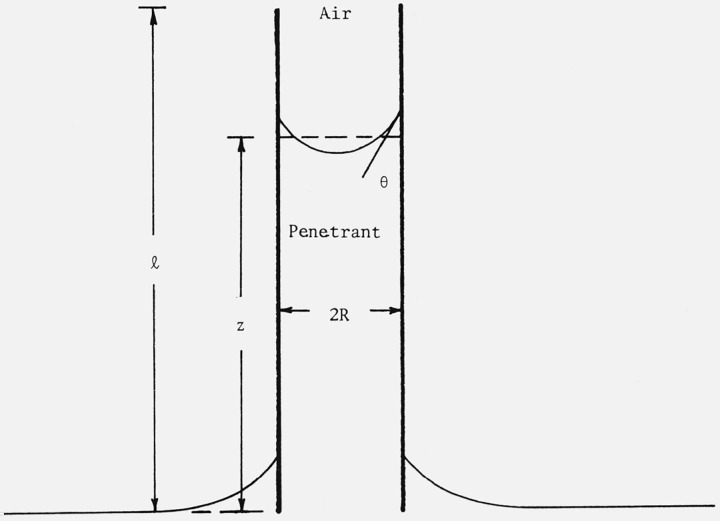
\includegraphics[width=0.55\textwidth]{figuras/deutsch-1979-flujo-capilar.jpg}
  \caption{Flujo capilar del penetrante en un tubo pequeño. Tomado de Deutsch
  (1979).}
  \label{fig:pt-flujo-capilar}
\end{figure}

Retirado el exceso de penetrante de la superficie, se aplica un medio poroso fino
llamado revelador. Éste se comporta como una esponja capilar inversa: absorbe el
líquido que quedó atrapado dentro de la fisura y forma una indicación visible cuyo
tamaño supera con creces el ancho real de la discontinuidad \parencite{almaguer2014}.
Por eso el método alcanza defectos muy por debajo de lo que distingue el ojo. La
Figura~\ref{fig:pt-falla} recoge una falla detectada de este modo en el espécimen 20
ensayado por Almaguer et al. (2014).

\begin{figure}[ht]
  \centering
  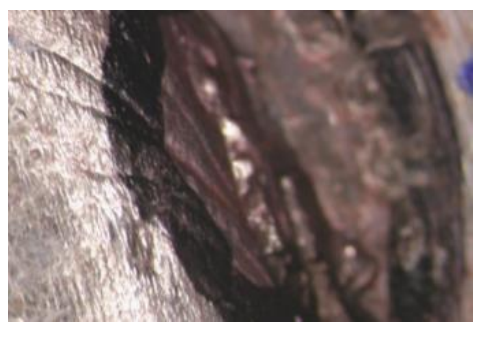
\includegraphics[width=0.42\textwidth]{figuras/almaguer-2014-falla-pt.png}
  \caption{Falla identificada por líquidos penetrantes en el espécimen 20. Adaptado
  de Almaguer et al. (2014).}
  \label{fig:pt-falla}
\end{figure}

\paragraph{Clasificación estandarizada del ensayo (ASTM E1417 / ISO 3452-1)}

De acuerdo con \parencite{astm_e1417, iso3452_1}, el proceso se clasifica según el
tipo de penetrante, el método de remoción del exceso y la forma del revelador.

\begin{enumerate}
  \item \textbf{Por tipo de penetrante:}
  \begin{itemize}
    \item \textbf{Tipo I (fluorescente):} contiene tintes fotosensibles que emiten
          fluorescencia verde-amarilla al excitarlos con radiación UV-A
          ($\lambda = 365\ \text{nm}$). Es el de mayor sensibilidad (niveles
          $1/2$ a $4$).
    \item \textbf{Tipo II (visible):} emplea colorantes rojos intensos que se
          observan con luz blanca natural o artificial ($\ge 1000\ \text{lux}$).
  \end{itemize}
  \item \textbf{Por método de remoción del exceso:}
  \begin{itemize}
    \item \textbf{lavable con agua}: el penetrante lleva agentes emulsionantes
          solubles en agua.
    \item \textbf{post-emulsionable lipofílico}: requiere aplicar después un
          emulsionante a base de aceite.
    \item \textbf{removible con solvente}: se elimina a mano con un paño impregnado
          en solvente no acuoso.
    \item \textbf{post-emulsionable hidrofílico}: usa un emulsionante diluido en agua
          antes del lavado final.
  \end{itemize}
  \item \textbf{Por forma de revelador:}
  \begin{itemize}
    \item polvo seco, aplicado en cámara de suspensión.
    \item soluble en agua.
    \item suspendible en agua.
    \item no acuoso para penetrante tipo I o II (aerosol con base de solvente).
  \end{itemize}
\end{enumerate}

\paragraph{Secuencia operativa estándar}

La inspección cuantitativa sigue seis etapas en orden \parencite{astm_e165}:

\begin{enumerate}
  \item \textbf{Limpieza previa.} Se quitan aceites, grasas, óxidos y pinturas
        mediante desengrase con solvente o ultrasonido.
  \item \textbf{Aplicación del penetrante y tiempo de morada.} Se aplica por
        inmersión, pulverización o pincel y se deja reposar entre $10$ y
        $30\ \text{min}$, según el material.
  \item \textbf{Remoción del exceso.} Se retira el penetrante de la superficie sin
        sacar el que quedó alojado dentro de los defectos.
  \item \textbf{Revelado.} Se extiende una capa delgada de revelador no acuoso
        (forma d) y se deja desarrollar al menos $10\ \text{min}$.
  \item \textbf{Inspección y evaluación.} Las indicaciones se interpretan en
        condiciones controladas: para el tipo II, con iluminación blanca
        $\ge 1000\ \text{lux}$; para el tipo I, con oscuridad ambiental
        ($\le 20\ \text{lux}$) e irradiancia UV-A
        $\ge 1000\ \mu\text{W/cm}^2$ a $38\ \text{cm}$ de distancia.
  \item \textbf{Limpieza posterior.} Se lava la pieza para evitar corrosión por
        residuos químicos.
\end{enumerate}

Con el penetrante se inspeccionan sin problema piezas de acero, de aluminio o de
titanio; también cerámicas y plásticos densos. La sensibilidad llega tan lejos que una
fisura de fatiga de menos de una micra se hace visible. Otra cosa son los materiales
porosos: en hormigón o en madera el líquido se reparte por toda la pieza y no deja una
indicación que se pueda localizar. Tampoco sirve para lo que está debajo de la
superficie, y una grieta tapada con grasa se pierde. Antes de empezar, conviene
limpiar.

\subsubsection{Inspección por partículas magnéticas (MT)}
\label{sec:mt}

\paragraph{Fundamentos}

La inspección por partículas magnéticas es un END de tipo magnetoelectrostático que
sirve para localizar discontinuidades superficiales y subsuperficiales en materiales
de alta permeabilidad magnética ($\mu_r \gg 1$): aceros al carbono, aceros de baja
aleación y fundiciones ferromagnéticas \parencite{astm_e1444, lovejoy1993}.

El punto de partida es la segunda ecuación de Maxwell, $\nabla \cdot \vec{B} = 0$,
que descarta la existencia de monopolos magnéticos \parencite{rao2012}. Si se induce
un flujo $\Phi$ en una pieza ferromagnética mediante una fuerza magnetomotriz
$\mathcal{F} = N I$, la reluctancia del circuito sigue la ley de Hopkinson
\parencite{lovejoy1993}:

\begin{equation}
  \mathcal{F} = \Phi\,\mathcal{R},
  \qquad
  \mathcal{R} = \frac{l}{\mu_0\,\mu_r\,A},
  \label{eq:hopkinson-reluctancia}
\end{equation}

donde $l$ es la longitud del trayecto magnético, $A$ el área de la sección
transversal, $\mu_0 = 4\pi\times10^{-7}\ \text{H/m}$ la permeabilidad del vacío y
$\mu_r$ la permeabilidad relativa ($100 \le \mu_r \le 5000$).

Cuando el flujo cruza perpendicularmente una fisura de apertura $w$ llena de aire o
de contaminantes ($\mu_{aire}\approx 1$), la reluctancia local sube de golpe
($\mathcal{R}_{grieta} \gg \mathcal{R}_{mat}$). Ese gradiente obliga a las líneas de
campo a deformarse y a salir por la superficie, lo que produce un campo disperso
conocido como fuga de flujo magnético (\textit{Magnetic Flux Leakage}, MFL)
\parencite{rao2012}. Las partículas ferromagnéticas que se espolvorean encima son
atraídas hacia las zonas de mayor gradiente de $|\vec{B}|^2$ por la fuerza Kelvin:

\begin{equation}
  \vec{F}_m = \frac{V_p\,\chi_m}{\mu_0}\,\nabla |\vec{B}|^2,
  \label{eq:fuerza-kelvin}
\end{equation}

con $V_p$ el volumen de la partícula y $\chi_m$ su susceptibilidad magnética.

\begin{figure}[ht]
\centering
\begin{tikzpicture}[scale=0.9]
  % pieza ferromagnética
  \fill[gray!12] (0,0) rectangle (8,2);
  \draw[thick] (0,0) rectangle (8,2);

  % líneas de campo dentro de la pieza
  \foreach \y in {0.3,0.7,1.1,1.5,1.9} {
    \draw[-{Stealth}] (0.25,\y) -- (7.75,\y);
  }

  % grieta llena de aire
  \fill[white] (3.85,0.8) rectangle (4.15,2);
  \draw[thick] (3.85,2) -- (3.85,0.8) -- (4.15,0.8) -- (4.15,2);

  % fuga de flujo magnético
  \draw[-{Stealth}] (3.85,2) .. controls (3.35,2.9) and (4.65,2.9) .. (4.15,2);
  \draw[-{Stealth}] (3.85,2) .. controls (3.55,3.45) and (4.45,3.45) .. (4.15,2);

  % yugo
  \draw[very thick] (1.5,2) -- (1.5,3.6) -- (6.5,3.6) -- (6.5,2);

  % bobina sobre la barra superior
  \foreach \x in {3.0,3.3,...,5.0} {
    \draw[thick] (\x,3.6) -- (\x,3.95);
  }
  \draw[thick] (2.9,3.95) -- (5.1,3.95);

  % partículas magnéticas
  \foreach \p in {(3.6,2.1),(3.75,2.22),(4.25,2.24),(4.4,2.1),(3.5,2.02),(4.5,2.02)} {
    \fill \p circle (0.05);
  }

  % etiquetas
  \node[left] at (1.35,2.9) {yugo};
  \node at (4,4.15) {bobina};
  \node[right,fill=white,inner sep=1pt] at (4.3,0.95) {grieta};
  \node[right,font=\small] at (4.85,2.55) {partículas};
  \draw[-{Stealth},thin] (4.85,2.5) -- (4.55,2.2);
  \node[below] at (4,-0.1) {pieza ferromagnética};
\end{tikzpicture}
\caption{Esquema del ensayo por partículas magnéticas: el yugo magnetiza la pieza,
la grieta distorsiona el campo y las partículas se acumulan en la fuga de flujo.}
\label{fig:mt-esquema}
\end{figure}

\paragraph{Efecto piel y selección del tipo de corriente}

La profundidad con que el campo entra en el material depende de la frecuencia $f$ de
la corriente de magnetización, por el efecto piel. Esa profundidad se estima como
\parencite{rao2012}

\begin{equation}
  \delta = \sqrt{\frac{\rho}{\pi f \mu_0 \mu_r}},
  \label{eq:efecto-piel}
\end{equation}

donde $\rho$ es la resistividad del material ($\Omega\cdot\text{m}$).

\begin{itemize}
  \item \textbf{Corriente alterna (AC, $50/60\ \text{Hz}$).} Como $\delta \approx
        1\ \text{mm}$ en aceros, el campo se queda en la capa superficial y da la
        mayor sensibilidad para fisuras por fatiga abiertas a la superficie.
  \item \textbf{Corriente continua (DC) o rectificada de media onda (HWDC).} Al
        anular la frecuencia ($f\to 0$), el campo penetra en toda la sección y
        permite detectar fisuras subsuperficiales de hasta $3$ a $6\ \text{mm}$.
\end{itemize}

\paragraph{Clasificación estandarizada y métodos (ASTM E1444 / ISO 9934-1)}

Según \parencite{astm_e1444, iso9934_1, asme_bpvc_v}, las técnicas de magnetización
y los medios de detección se ordenan así:

\begin{enumerate}
  \item \textbf{Técnicas de inducción del campo:}
  \begin{itemize}
    \item \textbf{Magnetización longitudinal (yugo o bobina):} el campo va paralelo
          al eje del yugo o del solenoide y detecta grietas transversales a ese eje.
    \item \textbf{Magnetización circular (paso de corriente o conductor central):}
          la corriente circula por la pieza o por un conductor central y genera un
          campo anular, apto para fisuras longitudinales.
    \item \textbf{Magnetización multidireccional:} aplica campos cruzados en
          secuencias rápidas y cubre cualquier orientación en una sola operación.
  \end{itemize}
  \item \textbf{Medios de detección:}
  \begin{itemize}
    \item \textbf{Método seco:} partículas finas de hierro u óxidos coloreados
          (negro, rojo, amarillo) sopladas con aire; sirve para campo y piezas
          rugosas o soldaduras.
    \item \textbf{Método húmedo:} partículas en suspensión en aceite ligero o en
          agua con inhibidor de corrosión.
  \end{itemize}
  \item \textbf{Contraste y visualización:}
  \begin{itemize}
    \item \textbf{Visibles:} se inspeccionan con luz blanca intensa
          ($\ge 1000\ \text{lux}$).
    \item \textbf{Fluorescentes:} llevan pigmentos que emiten verde-amarillo bajo
          UV-A ($\lambda = 365\ \text{nm}$).
  \end{itemize}
\end{enumerate}

\paragraph{Verificación del yugo y secuencia operativa}

La validez del ensayo exige comprobar periódicamente la fuerza del yugo
(\textit{Yoke Lift Test}) conforme a ASTM E1444 \parencite{astm_e1444}:

\begin{itemize}
  \item \textbf{Yugo de AC:} debe levantar una placa patrón de acero de al menos
        $4.5\ \text{kg}$ ($10\ \text{lb}$) con la separación de polos de trabajo.
  \item \textbf{Yugo de DC:} debe levantar al menos $18.1\ \text{kg}$
        ($40\ \text{lb}$).
\end{itemize}

La secuencia estándar tiene estas fases \parencite{iso9934_1}:

\begin{enumerate}
  \item \textbf{Preparación de la superficie.} Se limpian grasa, escamas de
        laminación, pintura suelta y residuos magnéticos.
  \item \textbf{Posicionamiento del yugo y magnetización.} Los polos se apoyan
        perpendiculares a la dirección esperada de la grieta.
  \item \textbf{Aplicación continua de partículas.} El medio húmedo o seco se
        dispersa mientras la corriente sigue activa (\textit{método continuo}).
  \item \textbf{Inspección visual y evaluación.} Con partículas visibles se requiere
        $\ge 1000\ \text{lux}$; con fluorescentes, oscuridad ambiental
        $\le 20\ \text{lux}$ e irradiancia UV-A
        $\ge 1000\ \mu\text{W/cm}^2$ a $38\ \text{cm}$.
  \item \textbf{Desmagnetización residual.} Se aplica un campo alterno decreciente e
        invertido para bajar la inducción remanente de $0.3\ \text{mT}$
        ($3\ \text{Gauss}$) \parencite{astm_e1444}.
\end{enumerate}

El yugo es rápido de usar y el equipo no cuesta mucho. Con corriente continua o
rectificada se ven grietas que no salen a la superficie, hasta unos milímetros
adentro, y la indicación queda justo donde está el defecto; sobre esas imágenes se han
probado algoritmos de segmentación para automatizar la lectura
\parencite{ueda2021}. Ahora bien, si el material no es ferromagnético no hay caso: en
inoxidable austenítico, aluminio o titanio el yugo no genera fuga. Y al terminar toca
desmagnetizar, sobre todo en piezas de aviación o engranajes.

\subsubsection{Inspección por ultrasonido (UT) y medición de espesores}
\label{sec:ut}

\paragraph{Fundamentos}

La inspección por ultrasonido es un método volumétrico de END que se apoya en la
propagación de ondas elásticas de alta frecuencia ($0.5$ a $25\ \text{MHz}$) por
medios sólidos homogéneos \parencite{krautkramer1990, iso16810}.

En un sólido elástico e isótropo, la velocidad de una onda longitudinal $c_L$ depende
del módulo de Young $E$, del coeficiente de Poisson $\nu$ y de la densidad $\rho$
\parencite{cheeke2017}:

\begin{equation}
  c_L = \sqrt{\frac{E(1-\nu)}{\rho(1+\nu)(1-2\nu)}}.
  \label{eq:velocidad-longitudinal}
\end{equation}

Para el acero al carbono a $20\ ^\circ\text{C}$ se tiene $c_L \approx
5920\ \text{m/s}$.

La medición de espesores por eco de pulso (\textit{pulse-echo}) consiste en medir el
tiempo de vuelo de ida y vuelta, $\Delta t$, que tarda el pulso en ir de la superficie
de entrada a la pared posterior (o a una discontinuidad) y volver al receptor
\parencite{astm_e797}:

\begin{equation}
  d = \frac{c_L\,\Delta t}{2}.
  \label{eq:espesor-tof}
\end{equation}

Al llegar a la interfaz entre el material ($Z_1$) y el medio exterior o la grieta
($Z_2$), la onda se refleja y se refracta según la diferencia de impedancia acústica
$Z = \rho c_L$ ($\text{Pa}\cdot\text{s/m}$). El coeficiente de reflexión en
intensidad, en incidencia normal, es \parencite{krautkramer1990}

\begin{equation}
  R = \left(\frac{Z_2 - Z_1}{Z_2 + Z_1}\right)^2.
  \label{eq:coeficiente-reflexion}
\end{equation}

En la interfaz acero-aire ($Z_{acero}\approx 45\times10^6\ \text{Pa}\cdot\text{s/m}$
frente a $Z_{aire}\approx 400\ \text{Pa}\cdot\text{s/m}$), $R\approx 0.9999$: casi
toda la energía ($99.99\%$) vuelve, lo que permite detectar grietas y medir
espesores con buena resolución.

\paragraph{Acoplamiento acústico y transductores piezoeléctricos}

El pulso se genera y se recibe por efecto piezoeléctrico inverso y directo en
cristales sintéticos de titanato zirconato de plomo (PZT) o niobato de litio
\parencite{cheeke2017}.

\begin{itemize}
  \item \textbf{Transductores de elemento dual.} Llevan dos cristales independientes
        sobre suelas en ángulo, uno emisor y otro receptor, separados por una barrera
        de aislamiento acústico. Así se elimina el ruido de campo cercano y la zona
        muerta, lo que mejora la medición de espesores delgados
        ($0.8$ a $50\ \text{mm}$) y la detección de corrosión interna (picaduras)
        \parencite{astm_e797}.
  \item \textbf{Acoplante acústico.} Como el aire en la interfaz sonda-pieza bloquea
        la onda ($R\to 1$), se aplica un fluido o gel (glicerina, gel acuoso o aceite
        mineral) que elimina la película de aire y deja pasar el pulso.
\end{itemize}

\paragraph{Procedimiento de calibración según INACAL PC-029}

La calibración de un medidor digital de espesores por ultrasonido (por ejemplo, el
INSIZE ISU-100D, resolución $0.01\ \text{mm}$) sigue el procedimiento INACAL PC-029
\parencite{inacal_pc029, astm_e797}:

\begin{enumerate}
  \item \textbf{Ajuste del cero del palpador.} Se compensa el retardo acústico que
        introduce la suela del transductor.
  \item \textbf{Ajuste de la velocidad del sonido.} El instrumento se calibra con un
        bloque patrón de acero a dos espesores acotados, por ejemplo
        $L_1 = 2.5\ \text{mm}$ y $L_2 = 20.0\ \text{mm}$.
  \item \textbf{Verificación de linealidad.} Se evalúan cinco puntos uniformes de un
        bloque patrón escalonado (\textit{step block}) con trazabilidad nacional o
        internacional.
  \item \textbf{Incertidumbre combinada.} Conforme a la guía GUM
        \parencite{jcgm2008gum}, la incertidumbre del espesor medido se compone de
        \begin{equation}
          u_c^2(d) = u^2(\bar{d}_{rep}) + u^2(d_{res}) + u^2(L_{BP})
                     + u^2(\delta c_L) + u^2(\delta T),
          \label{eq:ut-incertidumbre}
        \end{equation}
        donde $u(\bar{d}_{rep}) = s/\sqrt{n}$ es la repetibilidad (tipo A),
        $u(d_{res}) = d_{res}/(2\sqrt{3})$ la resolución del display y
        $u(\delta c_L)$ recoge la variabilidad del material.
\end{enumerate}

\paragraph{Modos de presentación de datos ultrasónicos}

La Figura~\ref{fig:ut-modos} resume los tres modos con que se presenta la señal.

\begin{figure}[ht]
\centering
\begin{tikzpicture}[scale=0.82]
  % (a) A-Scan
  \begin{scope}
    \draw[-{Stealth}] (0,0) -- (4.2,0) node[right,font=\scriptsize] {$t$};
    \draw[-{Stealth}] (0,0) -- (0,2.2) node[above,font=\scriptsize] {$A$};
    \draw[thick] (0.15,0.1) -- (3.9,0.1);
    \draw[thick] (0.35,0.1) -- (0.45,1.55) -- (0.55,0.1);
    \draw[thick] (0.65,0.1) -- (0.8,0.28) -- (0.95,0.08)
                 -- (1.1,0.24) -- (1.25,0.07) -- (1.4,0.2)
                 -- (1.55,0.06) -- (1.7,0.16) -- (1.85,0.05)
                 -- (2.0,0.13) -- (2.15,0.04) -- (2.3,0.1) -- (2.45,0.05);
    \draw[thick] (2.65,0.05) -- (2.75,1.15) -- (2.85,0.05);
    \node[font=\scriptsize] at (2.1,-0.55) {(a) A-Scan};
  \end{scope}

  % (b) B-Scan
  \begin{scope}[shift={(5.3,0)}]
    \fill[gray!12] (0,0) rectangle (4,2);
    \draw (0,0) rectangle (4,2);
    \fill[gray!55] (0,1.55) rectangle (4,1.75);
    \fill[black!80] (2.1,0.55) rectangle (2.45,0.85);
    \draw[-{Stealth}] (0,-0.15) -- (4.2,-0.15) node[right,font=\scriptsize] {$x$};
    \draw[-{Stealth}] (-0.15,0) -- (-0.15,2.15) node[above,font=\scriptsize] {$t$};
    \node[font=\scriptsize] at (2.1,-0.55) {(b) B-Scan};
  \end{scope}

  % (c) C-Scan
  \begin{scope}[shift={(10.6,0)}]
    \fill[gray!10] (0,0) rectangle (4,2);
    \draw (0,0) rectangle (4,2);
    \fill[red!20] (2.0,0.9) circle (0.55);
    \fill[red!60] (2.0,0.9) circle (0.3);
    \draw[-{Stealth}] (0,-0.15) -- (4.2,-0.15) node[right,font=\scriptsize] {$x$};
    \draw[-{Stealth}] (-0.15,0) -- (-0.15,2.15) node[above,font=\scriptsize] {$y$};
    \node[font=\scriptsize] at (2.1,-0.55) {(c) C-Scan};
  \end{scope}
\end{tikzpicture}
\caption{Modos de presentación de datos ultrasónicos: (a) A-Scan, amplitud frente al
tiempo de vuelo; (b) B-Scan, corte transversal con la indicación del defecto;
(c) C-Scan, vista en planta con la posición del reflector.}
\label{fig:ut-modos}
\end{figure}

\begin{itemize}
  \item \textbf{A-Scan (amplitud).} Gráfica unidimensional de la señal RF o
        rectificada: la amplitud del eco ($y$) frente al tiempo de vuelo o la
        distancia ($x$).
  \item \textbf{B-Scan (corte transversal).} Representación bidimensional del perfil
        de la pieza a lo largo de una línea de escaneo; sirve para ver mapas de
        corrosión y pérdida de pared.
  \item \textbf{C-Scan (vista de planta).} Mapeo en el plano $x$-$y$ que muestra la
        profundidad o la amplitud de los reflectores en toda el área inspeccionada.
\end{itemize}

El ultrasonido atraviesa grandes espesores de acero y da centésimas de milímetro con
solo una cara accesible, sin fuentes de radiación que manipular. Los arreglos
multielemento permiten, además, construir los mapas B y C directamente
\parencite{drinkwater2006}. El punto flaco está en la preparación: sin acoplante el
pulso no entra, y si el bloque de referencia no es del mismo material la velocidad
introducida no sirve. Con geometrías raras o superficies rugosas, la lectura depende
demasiado de quien tiene la sonda en la mano.

\subsubsection{Inspección visual (VT)}
\label{sec:vt}

\paragraph{Fundamentos}

La inspección visual es el método primario de los END: se realiza antes que cualquier
otra técnica, superficial o volumétrica, y no necesita equipos especiales
\parencite{asme_bpvc_v_art9, iso17637}. Se apoya en la interacción de la luz visible
($\lambda \in [380,780]\ \text{nm}$) con la superficie de la pieza y en la respuesta
del ojo o de un sensor electroóptico \parencite{moore2012}.

La iluminación que llega al inspector sigue la ley del inverso del cuadrado de la
distancia y el teorema del coseno de Lambert \parencite{cheeke2017}:

\begin{equation}
  E_v = \frac{I_v \cos\theta}{r^2},
  \label{eq:iluminancia-lambert}
\end{equation}

donde $E_v$ es la iluminancia sobre la superficie ($\text{lux} = \text{lm/m}^2$),
$I_v$ la intensidad luminosa de la fuente (candela), $r$ la distancia de la fuente al
punto de inspección (m) y $\theta$ el ángulo entre la luz y la normal a la superficie.

La resolución espacial del ojo, $\Delta x_{min}$, se deduce del umbral de agudeza
visual angular $\theta_{min}\approx 1$ minuto de arco $= 2.91\times10^{-4}\ \text{rad}$
\parencite{moore2012}:

\begin{equation}
  \Delta x_{min} = d_{vis}\tan\theta_{min} \approx d_{vis}\,\theta_{min}.
  \label{eq:agudeza-visual}
\end{equation}

A la distancia de visión cercana, $d_{vis} = 250\ \text{mm}$, queda
$\Delta x_{min}\approx 0.07\ \text{mm}$ ($70\ \mu\text{m}$).

\paragraph{Clasificación estandarizada del ensayo (ISO 17637 / ASME Sec. V Art. 9)}

Conforme a \parencite{asme_bpvc_v_art9, iso17637}, la técnica se divide según la
accesibilidad de la pieza:

\begin{enumerate}
  \item \textbf{Inspección visual directa.} Se usa cuando hay línea de visión directa
        e ininterrumpida. Para asegurar la confiabilidad, las normas fijan la
        geometría de observación \parencite{iso17637}:
  \begin{itemize}
    \item \textbf{Distancia de visión:} el ojo no debe estar a más de
          $600\ \text{mm}$ ($24\ \text{pulg}$) de la superficie.
    \item \textbf{Ángulo de visión:} el ángulo entre la línea de visión y el plano de
          la superficie no debe ser menor de $30^\circ$.
    \item \textbf{Instrumentación auxiliar:} lupas de $2\times$ a $10\times$, espejos
          planos articulados, linternas LED de alta intensidad y galgas de soldadura
          (Cambridge, Hi-Lo, escala de filete y micrómetros de profundidad).
  \end{itemize}
  \item \textbf{Inspección visual remota o indirecta (RVT).} Se emplea en cavidades
        internas, tuberías de diámetro reducido, recipientes a presión o zonas de
        alta radiación donde no se puede acceder \parencite{asme_bpvc_v_art9}.
        Usa sistemas ópticos y optoelectrónicos:
  \begin{itemize}
    \item \textbf{Boroscopios rígidos:} lentes acromáticas en tubo metálico con guía
          de luz de fibra óptica; buena resolución angular, pero ángulo de visión
          fijo.
    \item \textbf{Fibroscopios flexibles:} haz de fibras ópticas coherentes para la
          imagen y fibras desordenadas para la iluminación.
    \item \textbf{Videoendoscopios digitales:} cabezales articulados con sensores
          micro-CCD/CMOS en la punta, iluminación LED y procesamiento digital, con
          medición tridimensional por estereofotogrametría o escaneo láser
          \parencite{moore2012}.
  \end{itemize}
\end{enumerate}

\begin{figure}[ht]
\centering
\begin{tikzpicture}[scale=0.85]
  % (a) inspección directa
  \begin{scope}
    \draw[thick] (0,0) -- (5,0);
    \draw[thick] (1.8,2.3) ellipse (0.4 and 0.25);
    \fill (1.8,2.3) circle (0.08);
    \draw[dashed] (1.8,2.05) -- (3.4,0);
    \draw (2.6,0) arc (180:128:0.8);
    \node[font=\scriptsize] at (2.7,0.45) {$\ge 30^\circ$};
    \node[font=\scriptsize] at (1.0,2.55) {ojo};
    % lupa
    \draw[thick] (3.9,1.1) circle (0.3);
    \draw[thick] (4.1,0.88) -- (4.3,0.68);
    \node[font=\scriptsize] at (3.9,1.55) {lupa};
    % defecto superficial
    \draw[thick] (3.1,0) -- (3.1,-0.22) -- (3.2,-0.22) -- (3.2,0);
    \node[font=\scriptsize] at (2.5,-0.55) {(a) directa};
  \end{scope}

  % (b) inspección remota
  \begin{scope}[shift={(7.5,0)}]
    \draw[thick] (0,0.3) -- (5,0.3) -- (5,2) -- (0,2) -- cycle;
    \draw[thick] (0.6,0.3) -- (0.6,2);
    \draw[very thick] (0.1,1.85) .. controls (1.2,1.85) and (1.4,1.4) .. (2.2,1.1);
    \fill (2.2,1.1) circle (0.1);
    \node[font=\scriptsize] at (2.55,1.25) {sonda};
    % cable y pantalla
    \draw[thick] (0.1,1.85) -- (-0.7,1.85);
    \draw[thick] (-1.7,1.2) rectangle (-0.7,2.3);
    \node[font=\scriptsize] at (-1.2,1.75) {pantalla};
    \node[font=\scriptsize] at (2.5,-0.55) {(b) remota};
  \end{scope}
\end{tikzpicture}
\caption{Inspección visual: (a) directa, con la línea de visión y el ángulo mínimo de
observación; (b) remota, con una sonda videoendoscópica en el interior de una
cavidad.}
\label{fig:vt-directa-remota}
\end{figure}

\paragraph{Secuencia operativa en uniones soldadas}

En uniones soldadas de acero estructural o tuberías, la inspección visual se hace en
tres fases \parencite{iso17637}:

\begin{enumerate}
  \item \textbf{Antes del soldeo.} Se verifica el ángulo de bisel, la apertura de
        raíz (\textit{root gap}), la alineación de bordes (\textit{hi-lo}), la
        ausencia de óxido, pintura o humedad y la conformidad de los materiales de
        aporte.
  \item \textbf{Durante el soldeo.} Se revisa la pasada de raíz, la limpieza de
        escoria entre pases y la posible aparición de grietas de solidificación o
        poros.
  \item \textbf{Después del soldeo.} Se evalúan la forma y el sobreespesor del
        refuerzo, las socavaciones (\textit{undercut}), la falta de llenado
        (\textit{underfill}), los traslapes (\textit{overlap}), las porosidades
        abiertas, las salpicaduras (\textit{spatter}) y el socavamiento de raíz.
\end{enumerate}

\paragraph{Requisitos ambientales y calificación del personal}

\begin{itemize}
  \item \textbf{Iluminancia.} ISO 17637 exige al menos $350\ \text{lux}$ sobre la
        superficie para inspección general y recomienda $1000\ \text{lux}$ para
        caracterizar microfisuras \parencite{iso17637}.
  \item \textbf{Calificación del inspector.} Debe acreditar cada año agudeza visual
        cercana con la carta Jaeger N.º 1 (o el equivalente ISO 18490 a
        $30\ \text{cm}$) y distinguir contrastes cromáticos (test de Ishihara),
        conforme a ISO 9712 o ASNT SNT-TC-1A \parencite{iso9712}.
\end{itemize}

Es el más barato de los ensayos: con una lupa y una linterna se descartan piezas mal
preparadas antes de meterse en un ensayo volumétrico. Pero solo alcanza lo que se ve;
una porosidad interna queda fuera. Y hay que contar con el factor humano: al final del
turno, con poca luz, el mismo defecto puede pasar. Por algo la norma se empeña en fijar
lux, distancia y ángulo.

\section{PROCEDIMIENTOS DE CALIBRACIÓN}
\subsection{PIE DE REY}
\label{sec:pie-de-rey}

\subsubsection{Instrumento, patrones y condiciones ambientales}

\begin{tabular}{ll}
Marca:      & Mitutoyo\\[3pt]
Código:     & 530-115\\[3pt]
Serie:      & 2013G454\\[3pt]
Resolución: & $0.05\text{ mm}$\\[3pt]
\end{tabular}

\vspace{6pt}
Procedimiento por comparación con instrumento de referencia según norma\\ PC-012 INACAL (\textit{Procedimiento de calibración de pie de rey}).

\vspace{12pt}
\subsubsection*{Equipos e instrumentos utilizados:}
\begin{tabular}{ll}
Bloques patrón de longitud & \\[3pt]
Cilindro patrón            & \\[3pt]
Anillo patrón              & \\[3pt]
Mesa de planitud           & \\[3pt]
Termómetro de contacto     & Exactitud $\pm 0.5\ ^\circ\text{C}$
\end{tabular}

\vspace{12pt}
\subsubsection*{Nomenclatura:}
\begin{tabular}{ll}
BU  & Bloques Utilizados\\[3pt]
VP  & Valor Patrón\\[3pt]
VPC & Valor Patrón Corregido\\[3pt]
PC  & Promedio Corregido\\[3pt]
$X_j$ & Lectura del pie de rey en la posición $j$ (superior, central, inferior)\\[3pt]
$D_j$ & Diferencia entre la lectura $j$ y el valor patrón corregido\\[3pt]
$E_k$ & Dispersión de las tres lecturas en el punto de calibración $k$\\[3pt]
$S_{E-I}$ & Error por cambio de la escala de exteriores a interiores\\[3pt]
$S_{E-P}$ & Error por cambio de la escala de exteriores a profundidad
\end{tabular}

\subsubsection{Datos experimentales}
\label{sec:pie-rey-datos}

Las mediciones se realizaron en cinco puntos distribuidos sobre el alcance del
instrumento, formando la pila de bloques patrón por acumulación: $50$ mm (un
bloque), $100$ mm (un bloque), $150$ mm (dos bloques), $200$ mm (tres bloques) y
$250$ mm (cuatro bloques). En cada punto se efectuaron tres mediciones
correspondientes a las posiciones superior, central e inferior de las mordazas de
medición de exteriores, conforme al ítem 10.1.2 de la norma PC-012. La temperatura
registrada fue de $21.5\ ^\circ$C en los cinco puntos, tal como se realizaron las
mediciones.

El pie de rey 530-115 es un instrumento de vernier cuya escala principal está
dividida en milímetros y cuyo nonio consta de 20 divisiones que abarcan 19 mm. La
diferencia entre una división de la escala principal y una del nonio define la
resolución del instrumento, $d = 1 - 19/20 = 0.05$ mm, de modo que toda lectura es
un múltiplo de dicha división. Las lecturas que se presentan a continuación respetan
esa graduación.

La Tabla~\ref{tab:pie-rey-datos} recoge las mediciones de los cinco puntos. La
columna BU indica los bloques que componen cada pila y la columna $VP$ el valor
nominal de la pila resultante.

\input{c3-calibration/pie-de-rey/tablas/t1.tex}

\subsubsection{Deducción de las ecuaciones de medición e incertidumbre}

Sea $F: \mathbb{R}^N \to \mathbb{R}$ una función aleatoria continua con densidad de
probabilidad conjunta $P(\vec{x})$ sobre $\Omega$, en el sentido de la
ecuación~\eqref{eq:mean-con-mult}, y sea $\vec{\mu} = (\mu_1, \dots, \mu_N)$ el
vector de valores medios $\mu_j = \bk{x_j}$. Conforme a la
ecuación~\eqref{eq:error-func}, $F$ puede expresarse como la suma de su valor medio
y una variación aleatoria $E(\vec{x})$, de modo que, aplicando la definición de la
ecuación~\eqref{eq:mean-con-mult},

\begin{align}
  F(\vec{x}) &= \bk{F} + E(\vec{x})
  \quad\Longrightarrow\quad
  E(\vec{x}) = F(\vec{x}) - \int_\Omega F(\vec{x})\,P(\vec{x})\,d^Nx ,
  \label{eq:modelo-base}
\end{align}

y de la ecuación~\eqref{eq:error-std} se sabe que $\bk{E} = 0$ y que
$\sigma_F^2 = \bk{E^2}$.

En el proceso de calibración interesa cuantificar el \textbf{error de indicación}.
Identificando la indicación media del pie de rey con $F(\vec{x}) \equiv L_i$ y el
valor de referencia del patrón con $\bk{F} \equiv L_{BP}$, la
ecuación~\eqref{eq:modelo-base} conduce a

\begin{equation}
  L_i = L_{BP} + E \quad\Longrightarrow\quad E = L_i - L_{BP},
  \label{eq:e-base}
\end{equation}

donde $L_i$ es el valor medio indicado por el pie de rey y $L_{BP}$ la longitud del
bloque patrón corregida por certificado. Esta expresión es análoga a la
ecuación~\eqref{eq:error-func} de la sección anterior.

\subsubsection*{Corrección por efectos térmicos}

Sea $T_0 = 20\ ^\circ\text{C}$ la temperatura de referencia y $\Delta T$ la
desviación de la temperatura de ensayo respecto de ella. Si $\alpha_i$ y
$\alpha_{BP}$ son los coeficientes de expansión térmica del pie de rey y del bloque
patrón, respectivamente, ambos cuerpos experimentan una dilatación lineal y la
ecuación~\eqref{eq:e-base} se corrige como

\begin{equation}
  E = L_i (1 + \alpha_i \Delta T_i) - L_{BP} (1 + \alpha_{BP} \Delta T_{BP}),
  \label{eq:e-termal}
\end{equation}

con $\Delta T_i = T_i - T_0$ y $\Delta T_{BP} = T_{BP} - T_0$. Expandiendo el
producto y agrupando términos,

\begin{align}
  E &= L_i + L_i \alpha_i \Delta T_i - L_{BP} - L_{BP} \alpha_{BP} \Delta T_{BP}
  \nonumber\\
  &= L_i - L_{BP} + L_i \alpha_i \Delta T_i - L_{BP} \alpha_{BP} \Delta T_{BP}.
  \label{eq:e-expanded}
\end{align}

Para separar el efecto del material del efecto del gradiente térmico se definen las
dos diferencias auxiliares

\begin{align}
  \delta\alpha &= \alpha_i - \alpha_{BP}, \label{eq:dalpha} \\
  \delta T &= \Delta T_i - \Delta T_{BP}, \label{eq:dT}
\end{align}

de las cuales $\alpha_i = \alpha_{BP} + \delta\alpha$ y
$\Delta T_{BP} = \Delta T_i - \delta T$. Sustituyendo en
\eqref{eq:e-expanded} y desarrollando,

\begin{align}
  E &= L_i + L_{BP}\left(\delta\alpha + \alpha_{BP}\right)\Delta T_i
     - L_{BP} + L_{BP}\alpha_{BP}\Delta T_i
     - L_{BP}\alpha_{BP}\Delta T_i \nonumber\\
  &\quad + L_{BP}\alpha_{BP}\,\delta T
     + \left(L_i - L_{BP}\right)\delta\alpha\,\Delta T_i .
\end{align}

El último término es proporcional al producto del error de indicación por dos
diferencias pequeñas, de modo que es de segundo orden. Despreciándolo y asumiendo la
proximidad dimensional $L_i \approx L_{BP}$ en los términos correctivos, se obtiene
el modelo de medición

\begin{equation}
  \therefore\quad
  E = L_i + L_i \, \delta\alpha \, \Delta T_i + L_{BP} \, \alpha_{BP} \, \delta T
  - L_{BP}.
  \label{eq:e-model}
\end{equation}

\subsubsection*{Relación funcional y cálculo de la incertidumbre combinada}

De la ecuación~\eqref{eq:e-model} se observa que $E$ es una función diferenciable
de seis variables de entrada,

\begin{equation}
  E = f(L_i; L_{BP}; \delta\alpha; \Delta T_i; \alpha_{BP}; \delta T),
  \label{eq:e-func}
\end{equation}

por lo que su varianza se obtiene aplicando la ley de propagación de la
ecuación~\eqref{eq:error-std-values}. Como las variables $x_j$ son estadísticamente
independientes, $\text{Cov}(x_i, x_j) = 0$ para $i \neq j$ y la suma se reduce a

\begin{equation}
  u_c^2(E) = \sum_{j=1}^6 \left. \left( \frac{\partial f}{\partial x_j}
  \right) \right|_{\vec{\mu}}^2 u^2(x_j),
  \label{eq:gum}
\end{equation}

donde los coeficientes de sensibilidad $\pti{f} = c_j$ se evalúan en el vector de
valores medios $\vec{\mu}$ según la ecuación~\eqref{eq:error-std-values}. Desarrollando
la sumatoria~\eqref{eq:gum} sobre las seis variables de entrada del
modelo~\eqref{eq:e-func}:

\begin{align}
  u_c^2(E) &=
  \left( \ptij{E}{L_i} \right)^2 u^2(L_i) +
  \left( \ptij{E}{L_{BP}} \right)^2 u^2(L_{BP}) \nonumber \\
  &\quad + \left( \ptij{E}{\delta\alpha} \right)^2 u^2(\delta\alpha) +
  \left( \ptij{E}{\Delta T_i} \right)^2 u^2(\Delta T_i) \label{eq:gum-expanded} \\
  &\quad + \left( \ptij{E}{\alpha_{BP}} \right)^2 u^2(\alpha_{BP}) +
  \left( \ptij{E}{\delta T} \right)^2 u^2(\delta T). \nonumber
\end{align}

Evaluando las derivadas parciales de la función~\eqref{eq:e-model} respecto a cada
variable de entrada:

\begin{align}
  \ptij{E}{L_i} &= 1 + \delta\alpha \, \Delta T_i, &
  \ptij{E}{L_{BP}} &= -1 + \alpha_{BP} \, \delta T, \nonumber \\
  \ptij{E}{\delta\alpha} &= L_i \, \Delta T_i, &
  \ptij{E}{\Delta T_i} &= L_i \, \delta\alpha, \label{eq:sens-deriv} \\
  \ptij{E}{\alpha_{BP}} &= L_{BP} \, \delta T, &
  \ptij{E}{\delta T} &= L_{BP} \, \alpha_{BP}. \nonumber
\end{align}

Sustituyendo los coeficientes~\eqref{eq:sens-deriv} en la
ecuación~\eqref{eq:gum-expanded} se obtiene la ecuación final para la varianza
combinada del error de indicación:

\begin{align}
  u_c^2(E) &=
  [1 + \delta\alpha \, \Delta T_i]^2 u^2(L_i) +
  [-1 + \alpha_{BP} \, \delta T]^2 u^2(L_{BP}) \nonumber \\
  &\quad + [L_i \, \Delta T_i]^2 u^2(\delta\alpha) +
  [L_i \, \delta\alpha]^2 u^2(\Delta T_i) \label{eq:sigma-final} \\
  &\quad + [L_{BP} \, \delta T]^2 u^2(\alpha_{BP}) +
  [L_{BP} \, \alpha_{BP}]^2 u^2(\delta T). \nonumber
\end{align}

\subsubsection{Reducción de datos y error de contacto de la superficie parcial}
\label{sec:pie-rey-reduccion}

Sea $T_k$ la temperatura registrada en el punto de calibración $k$ y
$T_0 = 20\ ^\circ\text{C}$ la temperatura de referencia. El valor de referencia de
cada punto es la longitud de la pila de bloques referida a $T_0$; por la
ecuación~\eqref{eq:e-termal}, e incorporando la corrección de certificado
$c_{cert,k}$,

\begin{align}
  VPC_k &= VP_k + c_{cert,k} + \alpha_{BP}\, L_k\,(T_k - T_0),
  \label{eq:vpc}
\end{align}

donde $VP_k$ es el valor nominal de la pila, $c_{cert,k}$ la corrección acumulada de
los bloques que la componen según su certificado,
$\alpha_{BP} = 11.5\times 10^{-6}\ ^\circ\text{C}^{-1}$ el coeficiente de expansión
térmica del acero de los bloques y $L_k \approx VP_k$. De forma análoga, la
indicación del pie de rey se refiere a $T_0$ según

\begin{equation}
  PC_{kj} = X_{kj}\left[1 - \alpha_i (T_k - T_0)\right],
  \label{eq:pc}
\end{equation}

donde $X_{kj}$ es la lectura en la posición $j$ del punto $k$.

El error de indicación de cada posición es la diferencia entre ambas reducciones.
Sustituyendo \eqref{eq:vpc} y \eqref{eq:pc} y desarrollando,

\begin{align}
  D_{kj} &= PC_{kj} - VPC_k \nonumber\\
  &= X_{kj} - X_{kj}\alpha_i (T_k - T_0) - VP_k - c_{cert,k}
     - \alpha_{BP}\,L_k (T_k - T_0). \label{eq:D-desarrollo}
\end{align}

Como $X_{kj} \approx L_k \approx VP_k$ en los términos correctivos y el pie de rey y
los bloques son de acero ($\alpha_i = \alpha_{BP} = \alpha$),

\begin{align*}
  D_{kj} &= X_{kj} - VP_k - c_{cert,k}
     - \alpha\,VP_k (T_k - T_0) + \alpha\,VP_k (T_k - T_0) \\
  &= X_{kj} - VP_k - c_{cert,k},
\end{align*}

es decir

\begin{equation}
  \therefore\quad D_{kj} \approx X_{kj} - VP_k - c_{cert,k},
  \label{eq:D}
\end{equation}

expresada en micrómetros. La corrección térmica se cancela por ser común a ambos
cuerpos, y la corrección de certificado es constante dentro de cada punto, de modo
que tampoco interviene en la dispersión: el error de contacto que se calcula a
continuación es independiente de $c_{cert,k}$ y de la corrección térmica.

La Tabla~\ref{tab:pie-rey-vpc} presenta, para cada punto, el valor patrón corregido,
el promedio corregido de las tres lecturas y el error de indicación resultante. Al no
disponer de las desviaciones certificadas de los bloques, se adopta $c_{cert,k} = 0$;
esta hipótesis no afecta al cálculo de $E$, pero sí al error de indicación reportado
en cada punto.

\input{c3-calibration/pie-de-rey/tablas/t2.tex}

\subsubsection*{Error de contacto de la superficie parcial en medición de exteriores}

Sea $E_k$ la dispersión de las tres posiciones en el punto $k$. El error de contacto
se define como la mayor de las dispersiones observadas,

\begin{equation}
  E = \max_k \left( \max_j D_{kj} - \min_j D_{kj} \right),
  \label{eq:E}
\end{equation}

cuyos valores se recogen en la Tabla~\ref{tab:pie-rey-diferencias}.

\input{c3-calibration/pie-de-rey/tablas/t3.tex}

Sustituyendo los valores de la Tabla~\ref{tab:pie-rey-diferencias}, la mayor
dispersión ($50\ \mu\text{m}$) aparece simultáneamente en los puntos de $100$ mm y
$200$ mm, de modo que el máximo de \eqref{eq:E} no es único. Conforme al criterio del
procedimiento, se selecciona el de mayor valor nominal:

\begin{equation}
  \therefore\quad E = 50\ \mu\text{m} \quad \text{en } 200 \text{ mm}.
  \label{eq:E-valor}
\end{equation}

Este resultado identifica además el punto crítico del instrumento para la prueba de
repetibilidad. Bajo el supuesto de una distribución rectangular de semiamplitud
$E/2$, la ecuación~\eqref{eq:sigma-rectangular} con $a = E/2$ proporciona

\begin{equation}
  \sigma(L_{i_E}) = \frac{2a}{2\sqrt{3}} = \frac{E}{2\sqrt{3}}
  = \frac{50}{2\sqrt{3}}\ \mu\text{m} \approx 14.43\ \mu\text{m}.
  \label{eq:sigma-LiE}
\end{equation}

% NOTACION: en todo el informe la incertidumbre típica se denota sigma(.),
% por continuidad con el marco teórico del capítulo 1. Equivale a u(.) en la
% notación de la GUM (JCGM 100:2008). Si más adelante se prefiere la notación
% GUM en la Tabla 6, el generador está en la celda del notebook que exporta
% t6.tex, en las líneas marcadas [GUM].

\paragraph{Estimación de las componentes de incertidumbre del pie de rey \texorpdfstring{$\sigma(L_i)$}{sigma(Li)}}
Para cuantificar las fuentes de variabilidad que afectan directamente la lectura del pie de rey, se evalúan las componentes geométricas, estadísticas y de resolución conforme al modelo de varianza de la ecuación~\eqref{eq:discrete-std-x-i}. Para cada componente acotada se aplica la distribución rectangular deducida en el marco teórico (ecuación~\eqref{eq:sigma-rectangular}), donde $\sigma = a/\sqrt{3}$ con $a$ la semiamplitud del intervalo.

La componente asociada al error de contacto de la superficie parcial, $\sigma(L_{i_E})$, se dedujo en la Sección~\ref{sec:pie-rey-reduccion} (ecuación~\eqref{eq:sigma-LiE}). A continuación se estiman las restantes.

\paragraph{Error de repetibilidad de contacto de la superficie parcial ($R$)}
Para cuantificar la dispersión aleatoria experimental (evaluación Tipo A), se seleccionan $n = 5$ mediciones repetidas en el punto de mayor error nominal. De acuerdo con las ecuaciones~\eqref{eq:std-s-eq} y~\eqref{eq:std-relative}, la desviación del promedio de $n$ observaciones independientes se reduce por el factor $1/\sqrt{n}$:

\begin{equation}
    \sigma(L_{i_R}) = \frac{s_R}{\sqrt{n}}
    \label{eq:sigma-LiR}
\end{equation}

donde la desviación estándar experimental de la muestra $s_R$ corresponde a:

\begin{equation}
    s_R = \sqrt{\frac{1}{n-1} \sum_{p=1}^n (R_p - \bar{R})^2}
    \label{eq:desv-estandar-muestral}
\end{equation}

siendo $R_p$ cada lectura individual y $\bar{R}$ la media aritmética muestral.

Las cinco repeticiones se efectuaron en el punto de $250$ mm, seleccionado por ser
el de mayor lectura de la serie (ante el empate en $E$ entre $100$ mm y $200$ mm se
optó por el extremo del alcance, donde el error de repetibilidad suele ser mayor):

\input{c3-calibration/pie-de-rey/tablas/t4.tex}

El rango de las cinco lecturas, $R = \max R_p - \min R_p = 50\ \mu\text{m}$, y la
desviación estándar experimental $s_R = 27.39\ \mu\text{m}$ conducen a

\begin{equation}
    \therefore\ \sigma(L_{i_R}) = \frac{27.39}{\sqrt{5}}\ \mu\text{m}
    \approx 12.25\ \mu\text{m}
    \label{eq:sigma-LiR-valor}
\end{equation}

Conviene notar que las cinco repeticiones fueron tomadas en una tanda distinta de
las mediciones de la Tabla~\ref{tab:pie-rey-datos}, donde las tres lecturas de
$250$ mm fueron $250.00$ mm. La diferencia de $0.08$ mm entre la media de las
repeticiones ($\bar{R} = 250.08$ mm) y aquella lectura refleja una deriva
instrumental entre ambas series, no dispersión aleatoria, y por ello no se suma a
$\sigma(L_i)$: la repetibilidad cuantifica únicamente la dispersión interna de la
tanda repetida, tal como define la ecuación~\eqref{eq:sigma-LiR}.

\paragraph{Error por cambio de escala ($S$)}
Representa la discrepancia al alternar entre la escala de medición de exteriores e interiores ($S_{E-I}$) o exteriores y profundidad ($S_{E-P}$). Tomando el caso más desfavorable $S = \max(S_{E-I}, S_{E-P})$ bajo el modelo de la ecuación~\eqref{eq:sigma-rectangular}:

\begin{equation}
    \sigma(L_{i_S}) = \frac{\max(S_{E-I}, S_{E-P})}{2\sqrt{3}}
    \label{eq:sigma-LiS}
\end{equation}

El ensayo se realizó sobre un cilindro patrón de $10$ mm, midiéndolo en tres
posiciones sobre la generatriz (superior, central e inferior) con cada una de las
tres aplicaciones del instrumento: exteriores, interiores y profundidad. La
Tabla~\ref{tab:pie-rey-cilindro} recoge las lecturas y los errores de indicación
correspondientes.

\input{c3-calibration/pie-de-rey/tablas/t5.tex}

Promediando las diferencias respecto de la medición de exteriores se obtiene
$S_{E-I} = 16.7\ \mu\text{m}$ y $S_{E-P} = 33.3\ \mu\text{m}$. El caso más
desfavorable es la medición de profundidad:

\begin{equation}
    \therefore\ \sigma(L_{i_S}) =
    \frac{33.3}{2\sqrt{3}}\ \mu\text{m} \approx 9.62\ \mu\text{m}
    \label{eq:sigma-LiS-valor}
\end{equation}

\paragraph{Errores geométricos de contacto y alineamiento ($L$, $J$, $K$)}
Siguiendo análogamente el modelo de la ecuación~\eqref{eq:sigma-rectangular}, las incertidumbres estándar por desviaciones de contacto y cruce resultan:

\begin{align}
    \sigma(L_{i_L}) &= \frac{L}{2\sqrt{3}} \label{eq:sigma-LiL} \\
    \sigma(L_{i_J}) &= \frac{J}{2\sqrt{3}} \label{eq:sigma-LiJ} \\
    \sigma(L_{i_K}) &= \frac{K}{2\sqrt{3}} \label{eq:sigma-LiK}
\end{align}

La medición del cilindro sobre la superficie de contacto lineal (aristas de las
mordazas sobre una generatriz) arrojó $L = 10\ \mu\text{m}$; sobre superficie
completa (bloques), $J = 0$; y en el cruce de las superficies de medición de
interiores, $K = 0$. Por tanto

\begin{equation}
    \sigma(L_{i_L}) = \frac{10}{2\sqrt{3}}\ \mu\text{m} \approx 2.89\ \mu\text{m},
    \qquad \sigma(L_{i_J}) = \sigma(L_{i_K}) = 0
    \label{eq:sigma-LiLJK-valor}
\end{equation}

\paragraph{Incertidumbre por resolución del pie de rey ($r$)}
El límite de discriminación instrumental define un intervalo de semiamplitud $\pm r/2$. Para escalas vernier se toma $r = d/m$ (con $d = 0.05\text{ mm}$, la división de escala del 530-115, y $m = 2$), obteniéndose mediante la ecuación~\eqref{eq:sigma-rectangular}:

\begin{equation}
    \sigma(L_{i_r}) = \frac{r}{\sqrt{3}} = \frac{d / m}{\sqrt{3}}
    \label{eq:sigma-Lir}
\end{equation}

Sustituyendo los valores del instrumento:

\begin{equation}
    \therefore\ \sigma(L_{i_r}) =
    \frac{0.05/2}{\sqrt{3}}\ \text{mm} \approx 14.43\ \mu\text{m}
    \label{eq:sigma-Lir-valor}
\end{equation}

\paragraph{Varianza combinada de la indicación $\sigma^2(L_i)$}
Asumiendo independencia estadística entre los factores evaluados ($\text{Cov} = 0$, conforme a la ecuación~\eqref{eq:error-std-values}), la varianza total de la indicación del pie de rey resulta de la suma en cuadratura de las ecuaciones~\eqref{eq:sigma-LiE} a~\eqref{eq:sigma-Lir}:

\begin{equation}
    \sigma^2(L_i) = \sigma^2(L_{i_E}) + \sigma^2(L_{i_R}) + \sigma^2(L_{i_S}) + \sigma^2(L_{i_L}) + \sigma^2(L_{i_J}) + \sigma^2(L_{i_K}) + \sigma^2(L_{i_r})
    \label{eq:sigma-Li-total}
\end{equation}

\subsubsection{Incertidumbre debida a los patrones de referencia \texorpdfstring{$\sigma(L_{BP})$}{sigma(LBP)}}

La longitud de referencia $L_{BP}$ incorpora dos contribuciones independientes:

\paragraph{Incertidumbre de calibración y combinación de bloques}
A partir de la incertidumbre expandida $U_{cal}$ reportada en el certificado para un factor de cobertura $k = 2$, la varianza combinada para una serie de $M$ bloques patrón acoplados es:

\begin{equation}
    \sigma^2(L_{BP_{cal}}) = \sum_{q=1}^M \left(\frac{U_{Lq,cal}}{k}\right)^2
    \label{eq:sigma-BP-cal}
\end{equation}

\paragraph{Deriva temporal de los bloques patrón}
Modelando la variación máxima permisible anual $U_{der}$ estipulada por la norma ISO 3650 mediante la distribución rectangular de la ecuación~\eqref{eq:sigma-rectangular}:

\begin{equation}
    \sigma^2(L_{BP_{der}}) = \sum_{q=1}^M \left(\frac{U_{Lq,der}}{\sqrt{3}}\right)^2
    \label{eq:sigma-BP-der}
\end{equation}

\paragraph{Varianza total del bloque patrón $\sigma^2(L_{BP})$}
Combinando ambas componentes independientes:

\begin{equation}
    \sigma^2(L_{BP}) = \sigma^2(L_{BP_{cal}}) + \sigma^2(L_{BP_{der}})
    \label{eq:sigma-LBP-total}
\end{equation}

El certificado de los bloques patrón no reporta una incertidumbre individual por
pieza, sino la expresión funcional con que el laboratorio la declara en función de
la longitud nominal $l$:

\begin{equation}
    U_{cal}(l) = 2\sqrt{a^2 + b^2 l^2},
    \qquad a = 41.46\ \text{nm},\quad b = 0.55\ \text{nm/mm},
    \label{eq:Ucal-bloque}
\end{equation}

con factor de cobertura $k = 2$. La deriva se estima con la variación máxima
permisible anual de la norma ISO~3650 para bloques de grado~1,
$U_{der}(l) = \pm(0.05\ \mu\text{m} + 0.5\times10^{-6}l)$. Evaluando ambas
expresiones sobre los cuatro bloques de la pila de $250$ mm ($25$, $50$, $75$ y
$100$ mm) resulta

\begin{equation}
    \sigma(L_{BP_{cal}}) = 0.1120\ \mu\text{m},
    \qquad \sigma(L_{BP_{der}}) = 0.0578\ \mu\text{m},
    \label{eq:sigma-BP-valor}
\end{equation}

\begin{equation}
    \therefore\ \sigma(L_{BP}) = \sqrt{0.1120^2 + 0.0578^2}\ \mu\text{m}
    \approx 0.126\ \mu\text{m}
    \label{eq:sigma-LBP-total-valor}
\end{equation}

\subsubsection{Incertidumbres asociadas a los parámetros térmicos}

Para las condiciones ambientales de ensayo, la temperatura registrada con el
termómetro de contacto fue de $21.5\ ^\circ\text{C}$ en los cinco puntos de
calibración (Tabla~\ref{tab:pie-rey-datos}), sin variación apreciable entre ellos. De
ahí resulta una desviación respecto de la temperatura de referencia de
$\Delta T_i = 21.5 - 20 = 1.5\ ^\circ\text{C}$, y una diferencia nula entre el bloque
patrón y el pie de rey, $\delta T = 0$, ya que ambos permanecieron en el mismo
ambiente durante la medición.

\paragraph{Coeficientes de dilatación térmica $\sigma^2(\alpha_{BP})$ y $\sigma^2(\delta\alpha)$}
Para bloques y pie de rey de acero con semiamplitudes de tolerancia $\Delta\alpha_{BP}$ y $\Delta\alpha_i$, la aplicación de la ecuación~\eqref{eq:sigma-rectangular} proporciona:

\begin{align}
    \sigma^2(\alpha_{BP}) &= \frac{\Delta\alpha_{BP}^2}{3}, \label{eq:sigma-alpha-BP} \\
    \sigma^2(\delta\alpha) &= \frac{\Delta\alpha_{BP}^2}{3} + \frac{\Delta\alpha_i^2}{3} \label{eq:sigma-dalpha}
\end{align}

El acero presenta $\alpha = 11.5\times10^{-6}\ ^\circ\text{C}^{-1}$ con una dispersión
de $\Delta\alpha = 1\times10^{-6}\ ^\circ\text{C}^{-1}$, igual para el bloque y para el
pie de rey por ser ambos del mismo material. Sustituyendo en las
ecuaciones~\eqref{eq:sigma-alpha-BP} y~\eqref{eq:sigma-dalpha}:

\begin{equation}
    \sigma(\alpha_{BP}) = \frac{1\times10^{-6}}{\sqrt{3}}\ ^\circ\text{C}^{-1}
    \approx 5.77\times10^{-7}\ ^\circ\text{C}^{-1}
    \label{eq:sigma-alpha-BP-valor}
\end{equation}

\begin{equation}
    \sigma(\delta\alpha) = \frac{\sqrt{2}\times10^{-6}}{\sqrt{3}}\ ^\circ\text{C}^{-1}
    \approx 8.16\times10^{-7}\ ^\circ\text{C}^{-1}
    \label{eq:sigma-dalpha-valor}
\end{equation}

\paragraph{Desviaciones y gradientes de temperatura $\sigma^2(\Delta T_i)$ y $\sigma^2(\delta T)$}
Para la desviación respecto de la temperatura de referencia intervienen la
incertidumbre del certificado del termómetro ($UT_{cert}/k$), la deriva instrumental
($UT_{der}/\sqrt{3}$), su resolución ($d_T / (m_T \sqrt{3})$) y la fluctuación
observada durante el ensayo ($\Delta t_{A_i}/\sqrt{3}$):

\begin{equation}
    \sigma^2(\Delta T_i) = \left(\frac{UT_{cert}}{k}\right)^2 + \frac{\Delta t_{A_i}^2}{3} + \left(\frac{d_T / m_T}{\sqrt{3}}\right)^2 + \frac{UT_{der}^2}{3}
    \label{eq:sigma-deltaTi}
\end{equation}

El termómetro de contacto del laboratorio tiene una exactitud de
$\pm 0.5\ ^\circ\text{C}$, una deriva de $0.5\ ^\circ\text{C}$ y una división de
escala $d_T = 0.2\ ^\circ\text{C}$ subdividida en $m_T = 5$ partes. Como la
temperatura registrada fue la misma en los cinco puntos, la fluctuación observada es
nula ($\Delta t_{A_i} = 0$). Sustituyendo en la ecuación~\eqref{eq:sigma-deltaTi}:

\begin{equation}
    \sigma(\Delta T_i) = \sqrt{\left(\frac{0.5}{2}\right)^2 + 0
    + \left(\frac{0.2/5}{\sqrt{3}}\right)^2 + \frac{0.5^2}{3}}\ ^\circ\text{C}
    \approx 0.383\ ^\circ\text{C}
    \label{eq:sigma-deltaTi-valor}
\end{equation}

De manera análoga, para el gradiente térmico diferencial entre los bloques y el pie de rey ($\delta T$):

\begin{equation}
    \sigma^2(\delta T) = \left(\frac{UT_{cert}}{k}\right)^2 + \frac{\Delta t^2}{3} + \left(\frac{d_T / m_T}{\sqrt{3}}\right)^2 + \frac{UT_{der}^2}{3}
    \label{eq:sigma-deltaT}
\end{equation}

donde $\Delta t = \max(\Delta t_1, \Delta t_2)$ representa la máxima diferencia térmica entre ambos cuerpos. Al haberse mantenido bloque y pie de rey en el mismo ambiente, esa diferencia también es nula, y por tanto

\begin{equation}
    \sigma(\delta T) \approx 0.383\ ^\circ\text{C}
    \label{eq:sigma-deltaT-valor}
\end{equation}

\paragraph{Contribución efectiva de los términos térmicos}
Las incertidumbres anteriores no se transmiten al resultado, porque los coeficientes
de sensibilidad que las multiplican en la ecuación~\eqref{eq:sigma-final} se anulan:
ambos cuerpos son de acero, de modo que $\delta\alpha = \alpha_i - \alpha_{BP} = 0$, y
ambos están a la misma temperatura, de modo que $\delta T = 0$. El único término
térmico que sobrevive es $[L_i\,\Delta T_i]^2 \sigma^2(\delta\alpha)$, que evaluado en
el extremo del alcance ($L_i = 250$ mm, $\Delta T_i = 1.5\ ^\circ\text{C}$) vale

\begin{equation}
    (250 \times 1.5)^2 \left(8.16\times10^{-7}\right)^2\ \mu\text{m}^2
    \approx 9.4\times10^{-8}\ \mu\text{m}^2,
    \label{eq:termino-termico}
\end{equation}

es decir diez órdenes de magnitud por debajo de $\sigma^2(L_i) = 667.6\ \mu\text{m}^2$.
Los parámetros térmicos son, en consecuencia, irrelevantes para la incertidumbre del
error de indicación de este instrumento en las condiciones de ensayo.

\subsubsection{Incertidumbre estándar combinada y expandida final}

Sustituyendo las componentes~\eqref{eq:sigma-Li-total},~\eqref{eq:sigma-LBP-total},~\eqref{eq:sigma-dalpha},~\eqref{eq:sigma-deltaTi} y~\eqref{eq:sigma-deltaT} en la ley de propagación de varianzas de la ecuación~\eqref{eq:sigma-final}, la varianza combinada del error de indicación queda expresada en forma completamente desarrollada como:

\begin{align}
    \sigma_c^2(E) &=
    [1 + \delta\alpha \, \Delta T_i]^2
    \Bigg[
        \left(\frac{E}{2\sqrt{3}}\right)^2
        + \frac{s_R^2}{n}
        + \left(\frac{\max(S_{E-I}, S_{E-P})}{2\sqrt{3}}\right)^2 \nonumber \\
    &\qquad\qquad
        + \left(\frac{L}{2\sqrt{3}}\right)^2
        + \left(\frac{J}{2\sqrt{3}}\right)^2
        + \left(\frac{K}{2\sqrt{3}}\right)^2
        + \left(\frac{d/m}{\sqrt{3}}\right)^2
    \Bigg] \nonumber \\[4pt]
    &\quad + [-1 + \alpha_{BP} \, \delta T]^2
    \Bigg[
        \sum_{q=1}^M \left(\frac{U_{Lq,cal}}{k}\right)^2
        + \sum_{q=1}^M \left(\frac{U_{Lq,der}}{\sqrt{3}}\right)^2
    \Bigg] \nonumber \\[4pt]
    &\quad + [L_i \, \Delta T_i]^2
    \Bigg[
        \frac{\Delta\alpha_{BP}^2}{3} + \frac{\Delta\alpha_i^2}{3}
    \Bigg] \nonumber \\[4pt]
    &\quad + [L_i \, \delta\alpha]^2
    \Bigg[
        \left(\frac{UT_{cert}}{k}\right)^2
        + \frac{\Delta t_{A_i}^2}{3}
        + \left(\frac{d_T / m_T}{\sqrt{3}}\right)^2
        + \frac{UT_{der}^2}{3}
    \Bigg] \nonumber \\[4pt]
    &\quad + [L_{BP} \, \delta T]^2
    \Bigg[
        \frac{\Delta\alpha_{BP}^2}{3}
    \Bigg] \nonumber \\[4pt]
    &\quad + [L_{BP} \, \alpha_{BP}]^2
    \Bigg[
        \left(\frac{UT_{cert}}{k}\right)^2
        + \frac{\Delta t^2}{3}
        + \left(\frac{d_T / m_T}{\sqrt{3}}\right)^2
        + \frac{UT_{der}^2}{3}
    \Bigg] \label{eq:sigma-cuad-expandida}
\end{align}

Finalmente, la incertidumbre expandida $U(E)$ para el error de indicación del pie de rey se reporta mediante:

\begin{equation}
    U(E) = k \cdot \sigma_c(E) = k \sqrt{\sigma_c^2(E)}
    \label{eq:incertidumbre-expandida}
\end{equation}

adoptando un factor de cobertura $k = 2$, correspondiente a un nivel de confianza bilateral aproximado del 95\,\%.


\subsubsection{Resultados numéricos de la calibración}
\label{sec:pie-rey-resultados}

Sustituyendo en la ley de propagación~\eqref{eq:sigma-final} las componentes
estimadas en las secciones anteriores se obtiene el balance de incertidumbres de la
indicación del pie de rey que se presenta en la
Tabla~\ref{tab:pie-rey-balance}.

\input{c3-calibration/pie-de-rey/tablas/t6.tex}

La varianza combinada de la indicación, conforme a la
ecuación~\eqref{eq:sigma-Li-total}, es la suma en cuadratura de las siete
contribuciones evaluadas:

\begin{equation}
    \sigma^2(L_i) = \sigma^2(L_{i_E}) + \sigma^2(L_{i_R}) + \sigma^2(L_{i_S})
    + \sigma^2(L_{i_L}) + \sigma^2(L_{i_J}) + \sigma^2(L_{i_K}) + \sigma^2(L_{i_r}),
    \label{eq:sigma-Li-simbolico}
\end{equation}

es decir

\begin{equation}
    \sigma^2(L_i) =
    \begin{aligned}
        &\left(\frac{E}{2\sqrt{3}}\right)^2
        + \left(\frac{s_R}{\sqrt{n}}\right)^2
        + \left(\frac{\max(S_{E-I}, S_{E-P})}{2\sqrt{3}}\right)^2
        + \left(\frac{L}{2\sqrt{3}}\right)^2 \\[4pt]
        &\quad + \left(\frac{J}{2\sqrt{3}}\right)^2
        + \left(\frac{K}{2\sqrt{3}}\right)^2
        + \left(\frac{d/m}{\sqrt{3}}\right)^2 .
    \end{aligned}
    \label{eq:sigma-Li-simbolico-exp}
\end{equation}

Sustituyendo los valores obtenidos para cada componente,

\begin{equation}
    \sigma^2(L_i) = (14.43)^2 + (12.25)^2 + (9.62)^2 + (2.89)^2 + 0 + 0 + (14.43)^2
    \ \mu\text{m}^2
    \label{eq:sigma-Li-num}
\end{equation}

\begin{equation}
    \therefore\ \sigma(L_i) \approx 25.84\ \mu\text{m}
    \label{eq:sigma-Li-num-valor}
\end{equation}

El error de indicación del pie de rey es prácticamente independiente del valor
patrón en las condiciones de trabajo: la diferencia de coeficientes de dilatación es
nula ($\delta\alpha = 0$, ambos de acero) y la diferencia de temperaturas entre el
bloque y el instrumento también lo es ($\delta T = 0$, ambos a $21.5\ ^\circ$C).
Evaluando la ecuación~\eqref{eq:sigma-cuad-expandida} con esos valores, los
coeficientes de sensibilidad $[1+\delta\alpha\,\Delta T_i]^2$ y
$[-1+\alpha_{BP}\,\delta T]^2$ toman el valor unidad, mientras que los términos
$[L_i\,\delta\alpha]^2$ y $[L_{BP}\,\delta T]^2$ se anulan por completo. Los dos
restantes, asociados a $\sigma^2(\delta\alpha)$ y a $\sigma^2(\alpha_{BP})$, no se
anulan pero resultan despreciables: el primero vale
$9.4\times10^{-8}\ \mu\text{m}^2$ en el extremo del alcance
(ecuación~\eqref{eq:termino-termico}) y el segundo es de orden $10^{-9}\ \mu\text{m}^2$,
frente a $\sigma^2(L_i) = 667.6\ \mu\text{m}^2$. Con esa aproximación, la
ecuación~\eqref{eq:sigma-cuad-expandida} se reduce a

\begin{equation}
    \sigma_c^2(E) = \sigma^2(L_i) + \sigma^2(L_{BP})
    \label{eq:sigma-c-num}
\end{equation}

Al desaparecer del modelo todos los términos que llevan la longitud como factor, la
varianza combinada deja de depender del valor nominal del punto de calibración. Si
se dejan explícitas las componentes térmicas de la
ecuación~\eqref{eq:sigma-cuad-expandida} como función de la longitud $L$, el modelo
completo conduce a la forma cerrada

\begin{equation}
    U(E,L) = \sqrt{8.343\times10^{-11}\,L^2 + 2670.4}\ \mu\text{m},
    \label{eq:U-vecL}
\end{equation}

con $L$ expresada en milímetros. El coeficiente del término cuadrático reúne el
aporte de los términos térmicos, que resulta despreciable: en el extremo del alcance
ensayado ($L = 250$ mm) contribuye con $9.4\times10^{-8}\ \mu\text{m}^2$ frente a los
$2670.4\ \mu\text{m}^2$ del término independiente, de modo que $U(E)$ permanece
constante en los cinco puntos de calibración.

Sustituyendo el valor de la ecuación~\eqref{eq:sigma-LBP-total-valor}:

\begin{equation}
    \sigma_c(E) = \sqrt{25.84^2 + 0.126^2}\ \mu\text{m}
    \approx 25.84\ \mu\text{m}
    \label{eq:sigma-c-num-valor}
\end{equation}

Finalmente, la incertidumbre expandida con factor de cobertura $k = 2$ resulta

\begin{equation}
    U(E) = 2 \times 25.84\ \mu\text{m} \approx 51.68\ \mu\text{m}
    \label{eq:U-num-valor}
\end{equation}

\subsubsection{Declaración de conformidad}

El error máximo permitido del pie de rey 530-115 especificado por el fabricante es
$\text{EMPE} = \pm 80\ \mu\text{m}$ para todo su alcance de $0$ a $300$ mm, aunque
el ensayo cubrió de $50$ a $250$ mm. Dado que

\begin{equation}
    U(E) \approx 51.68\ \mu\text{m} < \text{EMPE} = 80\ \mu\text{m},
    \qquad \frac{U(E)}{\text{EMPE}} \approx 0.65,
    \label{eq:conformidad}
\end{equation}

la incertidumbre de la calibración es menor que la tolerancia del instrumento, por
lo que el resultado permite decidir conformidad. Los cinco errores de indicación se
mantienen por debajo del EMPE, con un máximo de $+28.2\ \mu\text{m}$ en $150$ mm, el
$35$\,\% del límite permitido.

La conformidad es, por tanto, ajustada. Adoptando la banda de aceptación de
ILAC-G8, que exige $|E| \le \text{EMPE} - U \approx 28.3\ \mu\text{m}$, tres de los
cinco puntos caen holgadamente dentro, mientras que los de $150$ mm y $200$ mm
quedan en el borde de la zona de incertidumbre, donde el error está dentro de
tolerancia pero la incertidumbre del método impide afirmar conformidad sin riesgo.
El instrumento cumple, pero el margen disponible frente al EMPE es reducido y
conviene repetir la calibración si el instrumento sufre golpes o desgaste
apreciable.




\todo{Incorporar la sección de calibración por ultrasonido (3.3) cuando se disponga
de los datos experimentales.}

\section{Logros}

Durante el periodo de prácticas se consolidaron los siguientes resultados:

\begin{itemize}
  \item Se calibró el pie de rey Mitutoyo 530-115 en el intervalo de $50$ a
        $250\ \text{mm}$, con una incertidumbre expandida de
        $U(E) \approx 51.68\ \mu\text{m}$ ($k = 2$). El error máximo de indicación
        fue de $+28.2\ \mu\text{m}$ en $150\ \text{mm}$, inferior al
        $\text{EMPE} = \pm 80\ \mu\text{m}$ especificado por el fabricante, y la
        razón $U(E)/\text{EMPE} \approx 0.65$ permitió aplicar la regla de decisión
        para evaluar la conformidad punto por punto.
  \item Se calibró el comparador digital Mitutoyo ID-S1012M entre $1$ y
        $10\ \text{mm}$, obteniéndose un alcance de error de $5\ \mu\text{m}$ y una
        incertidumbre expandida que crece de $3.21$ a $3.33\ \mu\text{m}$ en todo el
        intervalo ensayado.
  \item Se aplicó de forma integrada la ley de propagación de incertidumbres
        desarrollada en el marco teórico, identificando las componentes dominantes
        en cada instrumento: la planitud de la mesa de soporte en el comparador, y
        el error de contacto y la resolución en el pie de rey.
  \item Se documentaron los cálculos en tablas y figuras que permiten reproducir
        cada etapa del análisis, desde los datos experimentales hasta la
        declaración de conformidad.
\end{itemize}

\section{Conclusiones}

\begin{itemize}
  \item Los dos instrumentos calibrados presentan errores de indicación dentro de la
        tolerancia especificada por el fabricante. En el pie de rey, no obstante, el
        margen respecto al $\text{EMPE}$ es reducido: dos de los cinco puntos quedan
        en la zona de incertidumbre de la regla ILAC-G8, por lo que se recomienda
        repetir la calibración ante golpes o desgaste apreciable.
  \item La incertidumbre expandida del pie de rey ($51.68\ \mu\text{m}$) está dominada
        por las componentes de contacto y resolución, mientras que los términos
        térmicos resultan despreciables al ser el bloque y el instrumento del mismo
        material y estar a la misma temperatura.
  \item En el reloj comparador la incertidumbre expandida es de
        $3.33\ \mu\text{m}$ en el extremo del alcance ensayado, con una dependencia
        muy débil de la longitud; la componente predominante es la planitud de la
        mesa de soporte.
  \item El desarrollo del marco teórico permitió conectar la estimación estadística
        de la repetibilidad con la evaluación tipo~B de las demás fuentes, y aplicar
        consistentemente la ley de propagación de errores a ambos procedimientos.
\end{itemize}

\todo{Completar con las conclusiones correspondientes a la calibración por
ultrasonido, cuando esa sección sea incorporada.}

\section{Anexos}
\todo{Agregar aquí los anexos: certificados de calibración, tablas de datos,
figuras y código de los notebooks.}

\addcontentsline{toc}{section}{\refname}
\printbibliography{}
\end{document}
